\chapter{Stochastic Expansion Methods}\label{uq:expansion}


%This chapter explores the polynomial chaos expansion (PCE) and
%stochastic collocation (SC) in greater detail than that provided in
%the uncertainty quantification chapter of the User's Manual.  
This chapter explores two approaches to forming stochastic expansions,
the polynomial chaos expansion (PCE), which employs bases of
multivariate orthogonal polynomials, and stochastic collocation (SC),
which employs bases of multivariate interpolation polynomials.  Both
approaches capture the functional relationship between a set of output
response metrics and a set of input random variables.

\section{Orthogonal polynomials} \label{uq:expansion:orth}

\subsection{Askey scheme} \label{uq:expansion:orth:askey}

Table~\ref{TAB:askey} shows the set of classical orthogonal
polynomials which provide an optimal basis for different continuous
probability distribution types.  It is derived from the family of
hypergeometric orthogonal polynomials known as the Askey
scheme~\cite{askey}, for which the Hermite polynomials originally
employed by Wiener~\cite{wiener} are a subset.  The optimality of
these basis selections derives from their orthogonality with respect
to weighting functions that correspond to the probability density
functions (PDFs) of the continuous distributions when placed in a
standard form.  The density and weighting functions differ by a
constant factor due to the requirement that the integral of the PDF
over the support range is one.

\begin{table}[h]
  \centering
  \caption{Linkage between standard forms of continuous probability distributions and Askey scheme of continuous hyper-geometric polynomials.}
  \label{TAB:askey} 
  \begin{tabular}{ccccc} \hline
   Distribution & Density function & Polynomial & Weight function & Support range \\ \hline \hline
   Normal      & $\frac{1}{\sqrt{2\pi}} e^{\frac{-x^2}{2}}$ & Hermite  $He_n(x)$ & $e^{\frac{-x^2}{2}}$ & $[-\infty, \infty]$ \\ \hline
   Uniform     & $\frac{1}{2}$ & Legendre $P_n(x)$ & $1$ & $[-1,1]$ \\ \hline
   Beta        & $ \frac{(1-x)^{\alpha}(1+x)^{\beta}}{2^{\alpha+\beta+1} B(\alpha+1,\beta+1)}$ & Jacobi   $P^{(\alpha,\beta)}_n(x)$ & $(1-x)^{\alpha}(1+x)^{\beta}$ & $[-1,1]$ \\ \hline
   Exponential & $e^{-x}$ & Laguerre $L_n(x)$ & $e^{-x}$ & $[0, \infty]$ \\ \hline
   Gamma       & $\frac{x^{\alpha} e^{-x}}{\Gamma(\alpha+1)}$ & Generalized Laguerre $L^{(\alpha)}_n(x)$ & $x^{\alpha} e^{-x}$ & $[0, \infty]$ \\ \hline \hline
  \end{tabular}
\end{table}

Note that Legendre is a special case of Jacobi for 
$\alpha = \beta = 0$, Laguerre is a special case of generalized 
Laguerre for $\alpha = 0$, $\Gamma(a)$ is the Gamma function which 
extends the factorial function to continuous values, and $B(a,b)$ is the 
Beta function defined as $B(a,b) = \frac{\Gamma(a)\Gamma(b)}{\Gamma(a+b)}$.
Some care is necessary when specifying the $\alpha$ and $\beta$
parameters for the Jacobi and generalized Laguerre polynomials since
the orthogonal polynomial conventions~\cite{abram_stegun} differ from
the common statistical PDF conventions.  The former conventions are
used in Table~\ref{TAB:askey}.

\subsection{Numerically generated orthogonal polynomials} 
\label{uq:expansion:orth:beyond_askey}

If all random inputs can be described using independent normal, 
uniform, exponential, beta, and gamma distributions, then Askey 
polynomials can be directly applied.  If correlation or other distribution
types are present, then additional techniques are required.  One
solution is to employ nonlinear variable transformations as described
in Section~\ref{uq:expansion:trans} such that an Askey basis can be 
applied in the transformed space.  This can be effective as shown
in~\cite{Eld07}, but convergence rates are typically degraded.  In
addition, correlation coefficients are warped by the nonlinear
transformation~\cite{Der86}, and simple expressions for these
transformed correlation values are not always readily available.  An
alternative is to numerically generate the orthogonal polynomials
(using Gauss-Wigert~\cite{simpson_gw}, discretized
Stieltjes~\cite{gautschi_book}, Chebyshev~\cite{gautschi_book}, or
Gramm-Schmidt~\cite{WillBijl06} approaches) and then compute their
Gauss points and weights (using the Golub-Welsch~\cite{GolubWelsch69}
tridiagonal eigensolution).  These solutions are optimal for given
random variable sets having arbitrary probability density functions and 
%preserve the exponential convergence rates for general UQ applications,
%and also eliminates the need to calculate correlation warping.
eliminate the need to induce additional nonlinearity through variable
transformations, but performing this process for general joint density
functions with correlation is a topic of ongoing research (refer to
Section~\ref{uq:expansion:trans} for additional details).

\section{Interpolation polynomials} \label{uq:expansion:interp}

Interpolation polynomials may be either local or global and either
value-based or gradient-enhanced: Lagrange (global value-based),
Hermite (global gradient-enhanced), piecewise linear spline (local
value-based), and piecewise cubic spline (local gradient-enhanced).
Each of these combinations can be used within nodal or hierarchical
interpolation formulations.  The subsections that follow describe the
one-dimensional interpolation polynomials for these cases and
Section~\ref{uq:expansion:sc} describes their use for multivariate
interpolation within the stochastic collocation algorithm.

\subsection{Nodal interpolation} \label{uq:expansion:interp:nodal}

For value-based interpolation of a response function $R$ in one
dimension at an interpolation level $l$ containing $m^l$ points, the
expression
\begin{equation}
R(\xi) \cong I^l(R) = \sum_{j=1}^{m_l} r(\xi_j)\,L_j(\xi) \label{eq:lagrange_interp_1d}
\end{equation}
reproduces the response values $r(\xi_j)$ at the interpolation points
and smoothly interpolates between these values at other points.  As we
refine the interpolation level, we increase the number of collocation 
points in the rule and the number of interpolated response values.

For the case of gradient-enhancement, interpolation of a 
one-dimensional function
involves both type 1 and type 2 interpolation polynomials,
\begin{equation}
R(\xi) \cong I^l(R) = \sum_{j=1}^{m_l} \left[ r(\xi_j) H_j^{(1)}(\xi) + 
  \frac{dr}{d\xi}(\xi_j) H_j^{(2)}(\xi) \right] \label{eq:hermite_interp_1d}
\end{equation}
where the former interpolate a particular value while producing a zero
gradient ($i^{th}$ type 1 interpolant produces a value of 1 for the
$i^{th}$ collocation point, zero values for all other points, and zero
gradients for all points) and the latter interpolate a particular
gradient while producing a zero value ($i^{th}$ type 2 interpolant
produces a gradient of 1 for the $i^{th}$ collocation point, zero
gradients for all other points, and zero values for all points).


\subsubsection{Global value-based} \label{uq:expansion:interp:Lagrange}

Lagrange polynomials interpolate a set of points in a single dimension
using the functional form
\begin{equation}
L_j = \prod_{\stackrel{\scriptstyle k=1}{k \ne j}}^m 
\frac{\xi - \xi_k}{\xi_j - \xi_k} \label{eq:lagrange_poly_1d}
\end{equation}
where it is evident that $L_j$ is 1 at $\xi = \xi_j$, is 0 for each of
the points $\xi = \xi_k$, and has order $m - 1$.  

To improve numerical efficiency and stability, a barycentric Lagrange
formulation~\cite{BerTref04,Higham04} is used.  We define
the barycentric weights $w_j$ as
\begin{equation}
w_j = \prod_{\stackrel{\scriptstyle k=1}{k \ne j}}^m 
\frac{1}{\xi_j - \xi_k} \label{eq:barycentric_weights}
\end{equation}
and we precompute them for a given interpolation point set 
$\xi_j, j \in 1, ..., m$.  Then, defining the quantity $l(\xi)$ as
\begin{equation}
l(\xi) = \prod_{k=1}^m (\xi - \xi_k) \label{eq:barycentric_prod}
\end{equation}
which will be computed for each new interpolated point $\xi$, we can 
rewrite Eq.~\ref{eq:lagrange_interp_1d} as
\begin{equation}
R(\xi) = l(\xi) \sum_{j=1}^m \frac{w_j}{x-x_j} r(\xi_j) 
\label{eq:barycentric_lagrange1_1d}
\end{equation}
where much of the computational work has been moved outside the
summation.  Eq.~\ref{eq:barycentric_lagrange1_1d} is the first form of
barycentric interpolation.  Using an identity from the interpolation
of unity ($R(\xi) = 1$ and each $r(\xi_j) = 1$ in
Eq.~\ref{eq:barycentric_lagrange1_1d}) to eliminate $l(x)$, we arrive
at the second form of the barycentric interpolation formula:
\begin{equation}
R(\xi) = 
\frac{\sum_{j=1}^m \frac{w_j}{x-x_j} r(\xi_j)}{\sum_{j=1}^m \frac{w_j}{x-x_j}}
\label{eq:barycentric_lagrange2_1d}
\end{equation}
For both formulations, we reduce the computational effort for
evaluating the interpolant from $O(m^2)$ to $O(m)$ operations per
interpolated point, with the penalty of requiring additional care to
avoid division by zero when $\xi$ matches one of the $\xi_j$.
Relative to the first form, the second form has the additional
advantage that common factors within the $w_j$ can be canceled
(possible for Clenshaw-Curtis and Newton-Cotes point sets, but not for
general Gauss points), further reducing the computational requirements.
Barycentric formulations can also be used for hierarchical
interpolation (Section~\ref{uq:expansion:interp:hierarch}) with
Lagrange interpolation polynomials, but they are not applicable to
local spline or gradient-enhanced Hermite interpolants.


\subsubsection{Global gradient-enhanced} \label{uq:expansion:interp:Hermite}

Hermite interpolation polynomials (not to be confused with Hermite
orthogonal polynomials shown in Table~\ref{TAB:askey}) interpolate
both values and derivatives.  In our case, we are interested in
interpolating values and first derivatives, i.e, gradients.
One-dimensional polynomials satisfying the interpolation constraints
for general point sets are generated using divided differences as
described in~\cite{Burk11}.

\subsubsection{Local value-based} \label{uq:expansion:interp:linear}

Linear spline basis polynomials define a ``hat function,'' 
which produces the value of one at its collocation point and decays 
linearly to zero at its nearest neighbors.  In the case where its
collocation point corresponds to a domain boundary, then the half
interval that extends beyond the boundary is truncated.

For the case of non-equidistant closed points (e.g., Clenshaw-Curtis),
the linear spline polynomials are defined as
\begin{equation}
L_j(\xi) = 
\begin{cases}
1 - \frac{\xi - \xi_j}{\xi_{j-1} - \xi_j} & 
\text{if $\xi_{j-1} \leq \xi \leq \xi_j$ (left half interval)}\\
1 - \frac{\xi - \xi_j}{\xi_{j+1} - \xi_j} & 
\text{if $\xi_j < \xi \leq \xi_{j+1}$ (right half interval)}\\
0 & \text{otherwise}
\end{cases}
\end{equation}

For the case of equidistant closed points (i.e., Newton-Cotes), this
can be simplified to
\begin{equation}
L_j(\xi) = 
\begin{cases}
1 - \frac{|\xi - \xi_j|}{h} & \text{if $|\xi - \xi_j| \leq h$}\\
0                           & \text{otherwise}
\end{cases}
\end{equation}
for $h$ defining the half-interval $\frac{b - a}{m - 1}$ of the hat
function $L_j$ over the range $\xi \in [a, b]$.  For the special case
of $m = 1$ point, $L_1(\xi) = 1$ for $\xi_1 = \frac{b+a}{2}$ in both 
cases above.

\subsubsection{Local gradient-enhanced} \label{uq:expansion:interp:cubic}

Type 1 cubic spline interpolants are formulated as follows:
\begin{equation}
H_j^{(1)}(\xi) = 
\begin{cases}
t^2(3-2t) ~~\text{for}~~ t = \frac{\xi-\xi_{j-1}}{\xi_j-\xi_{j-1}} & 
\text{if $\xi_{j-1} \leq \xi \leq \xi_j$ (left half interval)}\\
(t-1)^2(1+2t) ~~\text{for}~~ t = \frac{\xi-\xi_j}{\xi_{j+1}-\xi_j} &
\text{if $\xi_j < \xi \leq \xi_{j+1}$ (right half interval)}\\
0     & \text{otherwise}
\end{cases}
\end{equation}
which produce the desired zero-one-zero property for left-center-right
values and zero-zero-zero property for left-center-right gradients.  
Type 2 cubic spline interpolants are formulated as follows:
\begin{equation}
H_j^{(2)}(\xi) =
\begin{cases}
ht^2(t-1) ~~\text{for}~~ h = \xi_j-\xi_{j-1},~~ t = \frac{\xi-\xi_{j-1}}{h} & 
\text{if $\xi_{j-1} \leq \xi \leq \xi_j$ (left half interval)}\\
ht(t-1)^2 ~~\text{for}~~ h = \xi_{j+1}-\xi_j,~~ t = \frac{\xi-\xi_j}{h} &
\text{if $\xi_j < \xi \leq \xi_{j+1}$ (right half interval)}\\
0     & \text{otherwise}
\end{cases}
\end{equation}
which produce the desired zero-zero-zero property for left-center-right
values and zero-one-zero property for left-center-right gradients.  For 
the special case of $m = 1$ point over the range $\xi \in [a, b]$, 
$H_1^{(1)}(\xi) = 1$ and $H_1^{(2)}(\xi) = \xi$ for $\xi_1 = \frac{b+a}{2}$.

% TO DO: could add discussion of collocation weights

\subsection{Hierarchical interpolation} \label{uq:expansion:interp:hierarch}

In a hierarchical formulation, we reformulate the interpolation in
terms of differences between interpolation levels:
\begin{equation}
\Delta^l(R) = I^l(R) - I^{l-1}(R), ~~l \geq 1 \label{eq:interp_diff}
\end{equation}
where $I^l(R)$ is as defined in
Eqs.~\ref{eq:lagrange_interp_1d}--\ref{eq:hermite_interp_1d} using the 
same local or global definitions for $L_j(\xi)$, $H_j^{(1)}(\xi)$, and 
$H_j^{(2)}(\xi)$, and $I^{l-1}(R)$ is evaluated as $I^l(I^{l-1}(R))$, 
indicating reinterpolation of the lower level interpolant across the 
higher level point set~\cite{spinterp,AgaAlu09}.

Utilizing Eqs.~\ref{eq:lagrange_interp_1d}--\ref{eq:hermite_interp_1d},
we can represent this difference interpolant as
\begin{equation}
\Delta^l(R) = 
\begin{cases}
\sum_{j=1}^{m_l} \left[ r(\xi_j) - I^{l-1}(R)(\xi_j) \right] \,L_j(\xi) & 
\text{value-based}\\
\sum_{j=1}^{m_l} \left( \left[ r(\xi_j) - I^{l-1}(R)(\xi_j) \right] \,H^{(1)}_j(\xi)
+ \left[ \frac{dr}{d\xi}(\xi_j) - \frac{dI^{l-1}(R)}{d\xi}(\xi_j) \right] 
\,H^{(2)}_j(\xi) \right) & \text{gradient-enhanced}
\end{cases}
\label{eq:interp_diff_detail}
\end{equation}
where $I^{l-1}(R)(\xi_j)$ and $\frac{dI^{l-1}(R)}{d\xi}(\xi_j)$ are
the value and gradient, respectively, of the lower level interpolant
evaluated at the higher level points.  We then define hierarchical
surpluses ${s, s^{(1)}, s^{(2)}}$ at a point $\xi_j$ as the bracketed
terms in Eq~\ref{eq:interp_diff_detail}.  These surpluses can be
interpreted as local interpolation error estimates since they capture
the difference between the true values and the values predicted by the
previous interpolant.

For the case where we use nested point sets among the interpolation
levels, the interpolant differences for points contained in both sets
are zero, allowing us to restrict the summations above to
$\sum_{j=1}^{m_{\Delta_l}}$ where we define the set $\Xi_{\Delta_l} =
\Xi_l \setminus \Xi_{l-1}$ that contains $m_{\Delta_l} = m_l - m_{l-1}$ 
points.  $\Delta^l(R)$ then becomes
\begin{equation}
\Delta^l(R) = 
\begin{cases}
\sum_{j=1}^{m_{\Delta_l}} s(\xi_j)\,L_j(\xi)  & \text{value-based}\\
\sum_{j=1}^{m_{\Delta_l}} \left( s^{(1)}(\xi_j) \,H^{(1)}_j(\xi) 
+ s^{(2)}(\xi_j) \,H^{(2)}_j(\xi) \right) & \text{gradient-enhanced}
\end{cases}
\end{equation}
The original interpolant $I^l(R)$ can be represented as a summation
of these difference interpolants
\begin{equation}
I^l(R) = \Delta^l(R) + I^{l-1}(R) = \sum_{i=1}^{l} \Delta^l(R)
\end{equation}
We will employ these hierarchical definitions within stochastic
collocation on sparse grids in Section~\ref{uq:expansion:sc:hierarch}.


\section{Generalized Polynomial Chaos} \label{uq:expansion:pce}


The set of polynomials from \ref{uq:expansion:orth:askey}
and~\ref{uq:expansion:orth:beyond_askey} are used as an orthogonal basis to
approximate the functional form between the stochastic response output
and each of its random inputs.  The chaos expansion for a response $R$
takes the form
\begin{equation}
R = a_0 B_0 + \sum_{i_1=1}^{\infty} a_{i_1} B_1(\xi_{i_1}) + 
\sum_{i_1=1}^{\infty} \sum_{i_2=1}^{i_1} a_{i_1i_2} B_2(\xi_{i_1},\xi_{i_2}) +
\sum_{i_1=1}^{\infty} \sum_{i_2=1}^{i_1} \sum_{i_3=1}^{i_2} a_{i_1i_2i_3}
B_3(\xi_{i_1},\xi_{i_2},\xi_{i_3}) + ...\label{eq:expansion_long}
\end{equation}
where the random vector dimension is unbounded and each additional set
of nested summations indicates an additional order of polynomials in
the expansion.  This expression can be simplified by replacing the
order-based indexing with a term-based indexing
\begin{equation}
R = \sum_{j=0}^{\infty} \alpha_j \Psi_j(\boldsymbol{\xi})
\label{eq:expansion_short}
\end{equation}
where there is a one-to-one correspondence between $a_{i_1i_2...i_n}$
and $\alpha_j$ and between
$B_n(\xi_{i_1},\xi_{i_2},...,\xi_{i_n})$ and
$\Psi_j(\boldsymbol{\xi})$.  Each of the
$\Psi_j(\boldsymbol{\xi})$ are multivariate polynomials
which involve products of the one-dimensional polynomials.  For
example, a multivariate Hermite polynomial
$B(\boldsymbol{\xi})$ of order $n$ is defined from
\begin{equation}
B_n(\xi_{i_1}, ..., \xi_{i_n}) = 
e^{\frac{1}{2}\boldsymbol{\xi}^T\boldsymbol{\xi}} (-1)^n 
\frac{\partial^n}{\partial \xi_{i_1} ... \partial \xi_{i_n}} 
e^{-\frac{1}{2}\boldsymbol{\xi}^T\boldsymbol{\xi}} \label{eq:multivar_gen}
\end{equation}
which can be shown to be a product of one-dimensional Hermite polynomials
involving an expansion term multi-index $t_i^j$:
\begin{equation}
B_n(\xi_{i_1}, ..., \xi_{i_n}) = 
\Psi_j(\boldsymbol{\xi}) = 
\prod_{i=1}^{n} \psi_{t_i^j}(\xi_i) \label{eq:multivar_prod}
\end{equation}
%which provides a convenient form for sensitivity analysis as described
%in \ref{uq:expansion:rvsa}.
In the case of a mixed basis, the same multi-index definition is
employed although the one-dimensional polynomials $\psi_{t_i^j}$ are
heterogeneous in type.

\subsection{Expansion truncation and tailoring} \label{uq:expansion:pce:exp_tnt}

In practice, one truncates the infinite expansion at a finite number
of random variables and a finite expansion order
\begin{equation}
R \cong \sum_{j=0}^P \alpha_j \Psi_j(\boldsymbol{\xi})
\label{eq:pc_exp_trunc}
\end{equation}
Traditionally, the polynomial chaos expansion includes a complete
basis of polynomials up to a fixed total-order specification.  That is,
for an expansion of total order $p$ involving $n$ random variables, the 
expansion term multi-index defining the set of $\Psi_j$ is constrained by
\begin{equation}
\sum_{i=1}^{n} t_i^j \leq p \label{eq:to_multi_index}
\end{equation}
For example, the multidimensional basis polynomials for a second-order
expansion over two random dimensions are
\begin{eqnarray}
\Psi_0(\boldsymbol{\xi}) & = & \psi_0(\xi_1) ~ \psi_0(\xi_2) ~~=~~ 1 
\nonumber \\
\Psi_1(\boldsymbol{\xi}) & = & \psi_1(\xi_1) ~ \psi_0(\xi_2) ~~=~~ \xi_1 
\nonumber \\
\Psi_2(\boldsymbol{\xi}) & = & \psi_0(\xi_1) ~ \psi_1(\xi_2) ~~=~~ \xi_2 
\nonumber \\
\Psi_3(\boldsymbol{\xi}) & = & \psi_2(\xi_1) ~ \psi_0(\xi_2) ~~=~~ \xi_1^2 - 1 
\nonumber \\
\Psi_4(\boldsymbol{\xi}) & = & \psi_1(\xi_1) ~ \psi_1(\xi_2) ~~=~~ \xi_1 \xi_2 
\nonumber \\
\Psi_5(\boldsymbol{\xi}) & = & \psi_0(\xi_1) ~ \psi_2(\xi_2) ~~=~~ \xi_2^2 - 1 
\nonumber 
\end{eqnarray}
The total number of terms $N_t$ in an expansion of total order
$p$ involving $n$ random variables is given by
\begin{equation}
N_t ~=~ 1 + P ~=~ 1 + \sum_{s=1}^{p} {\frac{1}{s!}} \prod_{r=0}^{s-1} (n+r)
    ~=~ \frac{(n+p)!}{n!p!} \label{eq:num_to_terms}
\end{equation}
This traditional approach will be referred to as a ``total-order
expansion.''

An important alternative approach is to employ a ``tensor-product
expansion,'' in which polynomial order bounds are applied on a
per-dimension basis (no total-order bound is enforced) and all
combinations of the one-dimensional polynomials are included.  That
is, the expansion term multi-index defining the set of $\Psi_j$ is
constrained by
\begin{equation}
t_i^j \leq p_i \label{eq:tp_multi_index}
\end{equation}
where $p_i$ is the polynomial order bound for the $i^{th}$ dimension.
In this case, the example basis for $p = 2, n = 2$ is
\begin{eqnarray}
\Psi_0(\boldsymbol{\xi}) & = & \psi_0(\xi_1) ~ \psi_0(\xi_2) ~~=~~ 1 
\nonumber \\
\Psi_1(\boldsymbol{\xi}) & = & \psi_1(\xi_1) ~ \psi_0(\xi_2) ~~=~~ \xi_1 
\nonumber \\
\Psi_2(\boldsymbol{\xi}) & = & \psi_2(\xi_1) ~ \psi_0(\xi_2) ~~=~~ \xi_1^2 - 1
\nonumber \\
\Psi_3(\boldsymbol{\xi}) & = & \psi_0(\xi_1) ~ \psi_1(\xi_2) ~~=~~ \xi_2
\nonumber \\
\Psi_4(\boldsymbol{\xi}) & = & \psi_1(\xi_1) ~ \psi_1(\xi_2) ~~=~~ \xi_1 \xi_2 
\nonumber \\
\Psi_5(\boldsymbol{\xi}) & = & \psi_2(\xi_1) ~ \psi_1(\xi_2) ~~=~~ 
(\xi_1^2 - 1) \xi_2 \nonumber \\
\Psi_6(\boldsymbol{\xi}) & = & \psi_0(\xi_1) ~ \psi_2(\xi_2) ~~=~~ \xi_2^2 - 1 
\nonumber \\
\Psi_7(\boldsymbol{\xi}) & = & \psi_1(\xi_1) ~ \psi_2(\xi_2) ~~=~~ 
\xi_1 (\xi_2^2 - 1) \nonumber \\
\Psi_8(\boldsymbol{\xi}) & = & \psi_2(\xi_1) ~ \psi_2(\xi_2) ~~=~~ 
(\xi_1^2 - 1) (\xi_2^2 - 1) \nonumber
\end{eqnarray}
and the total number of terms $N_t$ is
\begin{equation}
N_t ~=~ 1 + P ~=~ \prod_{i=1}^{n} (p_i + 1) \label{eq:num_tp_terms}
\end{equation}

It is apparent from Eq.~\ref{eq:num_tp_terms} that the tensor-product
expansion readily supports anisotropy in polynomial order for each
dimension, since the polynomial order bounds for each dimension can be
specified independently.  It is also feasible to support anisotropy
with total-order expansions, through pruning polynomials that satisfy 
the total-order bound 
%(potentially defined from the maximum of the per-dimension bounds)
but violate individual per-dimension bounds (the number of these
pruned polynomials would then be subtracted from
Eq.~\ref{eq:num_to_terms}).  Finally, additional tailoring of the
expansion form is used in the case of sparse grids (see
Section~\ref{uq:expansion:spectral_sparse}) through the use of a
summation of anisotropic tensor expansions.
%Of particular interest is the tailoring of expansion form to target
%specific monomial coverage as motivated by the integration process
%employed for evaluating chaos coefficients.  If the specific monomial
%set that can be resolved by a particular integration approach is known
%or can be approximated, then the chaos expansion can be tailored to
%synchonize with this set.  Tensor-product and total-order expansions
%can be seen as special cases of this general approach (corresponding
%to tensor-product quadrature and Smolyak sparse grids with linear
%growth rules, respectively), whereas, for example, Smolyak sparse
%grids with nonlinear growth rules could generate synchonized expansion
%forms that are neither tensor-product nor total-order (to be discussed
%later in association with Figure~\ref{fig:pascal_sparse_lev4_Gauss}).
In all cases, the specifics of the expansion are codified in the
term multi-index, and subsequent machinery for estimating response 
values and statistics from the expansion
%(estimating response values at particular $\boldsymbol{\xi}$, evaluating
%response statistics by integrating over $\boldsymbol{\xi}$, etc.)
can be performed in a manner that is agnostic to the specific 
expansion form.


\section{Stochastic Collocation} \label{uq:expansion:sc}


The SC expansion is formed as a sum of a set of multidimensional
interpolation polynomials, one polynomial per interpolated response
quantity (one response value and potentially multiple response
gradient components) per unique collocation point.  

\subsection{Value-Based Nodal} \label{uq:expansion:sc:value}

For value-based interpolation in multiple dimensions, a tensor-product
of the one-dimensional polynomials described in
Section~\ref{uq:expansion:interp:Lagrange} or
Section~\ref{uq:expansion:interp:linear} is used:
\begin{equation}
R(\boldsymbol{\xi}) \cong \sum_{j_1=1}^{m_{i_1}}\cdots\sum_{j_n=1}^{m_{i_n}}
r\left(\xi^{i_1}_{j_1},\dots , \xi^{i_n}_{j_n}\right)\,
\left(L^{i_1}_{j_1}\otimes\cdots\otimes L^{i_n}_{j_n}\right)
\label{eq:lagrange_tensor}
\end{equation}
where $\boldsymbol{i} = (m_1, m_2, \cdots, m_n)$ are the number of
nodes used in the $n$-dimensional interpolation and $\xi_{j_k}^{i_k}$ 
indicates the $j^{th}$ point out of $i$ possible collocation points 
in the $k^{th}$ dimension.  This can be simplified to
\begin{equation}
R(\boldsymbol{\xi}) \cong \sum_{j=1}^{N_p} r_j \boldsymbol{L}_j(\boldsymbol{\xi})
\label{eq:lagrange_interp_nd}
\end{equation}
where $N_p$ is the number of unique collocation points in the
multidimensional grid.  The multidimensional interpolation polynomials
are defined as
\begin{equation}
\boldsymbol{L}_j(\boldsymbol{\xi}) = \prod_{k=1}^{n} L_{c_k^j}(\xi_k) 
\label{eq:multivar_L}
\end{equation}
where $c_k^j$ is a collocation multi-index (similar to the expansion
term multi-index in Eq.~\ref{eq:multivar_prod}) that maps from the
$j^{th}$ unique collocation point to the corresponding
multidimensional indices within the tensor grid, and we have dropped
the superscript notation indicating the number of nodes in each
dimension for simplicity.  The tensor-product structure preserves the
desired interpolation properties where the $j^{th}$ multivariate
interpolation polynomial assumes the value of 1 at the $j^{th}$ point
and assumes the value of 0 at all other points, thereby reproducing
the response values at each of the collocation points and smoothly
interpolating between these values at other unsampled points.  When
the one-dimensional interpolation polynomials are defined using a
barycentric formulation as described in
Section~\ref{uq:expansion:interp:Lagrange} (i.e., 
Eq.~\ref{eq:barycentric_lagrange2_1d}), additional efficiency in
evaluating a tensor interpolant is achieved using the procedure
in~\cite{Klimke05}, which amounts to a multi-dimensional extension to
Horner's rule for tensor-product polynomial evaluation.

Multivariate interpolation on Smolyak sparse grids involves a weighted
sum of the tensor products in Eq.~\ref{eq:lagrange_tensor} with
varying $\boldsymbol{i}$ levels.  For sparse interpolants based on
nested quadrature rules (e.g., Clenshaw-Curtis, Gauss-Patterson,
Genz-Keister), the interpolation property is preserved, but sparse
interpolants based on non-nested rules may exhibit some interpolation
error at the collocation points.

%There is no need for tailoring of the expansion form as there is for
%PCE (i.e., to synchronize the expansion polynomials with the set of
%integrable monomials) since the polynomials that appear in the
%expansion are determined by the Lagrange construction
%(Eq.~\ref{eq:lagrange_poly_1d}).  That is, any tailoring or refinement
%of the expansion occurs through the selection of points in the
%interpolation grid and the polynomial orders of the basis are adapted
%implicitly.

\subsection{Gradient-Enhanced Nodal} \label{uq:expansion:sc:gradient}

For gradient-enhanced interpolation in multiple dimensions, we extend
the formulation in Eq~\ref{eq:lagrange_interp_nd} to use a
tensor-product of the one-dimensional type 1 and type 2 polynomials
described in Section~\ref{uq:expansion:interp:Hermite} or
Section~\ref{uq:expansion:interp:cubic}:
\begin{equation}
R(\boldsymbol{\xi}) \cong \sum_{j=1}^{N_p} \left[ 
r_j \boldsymbol{H}_j^{(1)}(\boldsymbol{\xi}) + 
\sum_{k=1}^n \frac{dr_j}{d\xi_k} \boldsymbol{H}_{jk}^{(2)}(\boldsymbol{\xi}) 
\right] \label{eq:hermite_interp_nd}
\end{equation}
The multidimensional type 1 basis polynomials are
\begin{equation}
\boldsymbol{H}_j^{(1)}(\boldsymbol{\xi}) =
\prod_{k=1}^{n} H^{(1)}_{c^j_k}(\xi_k) \label{eq:multivar_H1}
\end{equation}
where $c_k^j$ is the same collocation multi-index described for
Eq.~\ref{eq:multivar_L} and the superscript notation indicating the
number of nodes in each dimension has again been omitted.  The
multidimensional type 2 basis polynomials for the $k^{th}$ gradient
component are the same as the type 1 polynomials for each dimension
except $k$:
\begin{equation}
\boldsymbol{H}_{jk}^{(2)}(\boldsymbol{\xi}) = H^{(2)}_{c^j_k}(\xi_k)
\prod_{\stackrel{\scriptstyle l=1}{l \ne k}}^{n} H^{(1)}_{c^j_l}(\xi_l) 
\label{eq:multivar_H2}
\end{equation}

As for the value-based case, multivariate interpolation on Smolyak
sparse grids involves a weighted sum of the tensor products in
Eq.~\ref{eq:hermite_interp_nd} with varying $\boldsymbol{i}$ levels.

\subsection{Hierarchical} \label{uq:expansion:sc:hierarch}

In the case of multivariate hierarchical interpolation on nested grids, 
we are interested in tensor products of the one-dimensional difference
interpolants described in Section~\ref{uq:expansion:interp:hierarch},
with
\begin{equation}
\Delta^l(R) = \sum_{j_1=1}^{m_{\Delta_1}}\cdots\sum_{j_n=1}^{m_{\Delta_n}}
s\left(\xi^{\Delta_1}_{j_1},\dots , \xi^{\Delta_n}_{j_n}\right)\,
\left(L^{\Delta_1}_{j_1}\otimes\cdots\otimes L^{\Delta_n}_{j_n}\right)
\label{eq:hierarch_interp_nd_L}
\end{equation}
for value-based, and
\begin{eqnarray}
& \Delta^l(R) & =
\sum_{j_1=1}^{m_{\Delta_1}} \cdots \sum_{j_n=1}^{m_{\Delta_n}} \nonumber \\
& & \left[ 
s^{(1)} \left( \xi^{\Delta_1}_{j_1}, \dots, \xi^{\Delta_n}_{j_n} \right)
\left( H^{(1)~\Delta_1}_{~~~~~j_1} \otimes \cdots \otimes H^{(1)~\Delta_n}_{~~~~~j_n}
\right) + \sum_{k=1}^n s_k^{(2)} \left(\xi^{\Delta_1}_{j_1}, \dots, \xi^{\Delta_n}_{j_n}\right)
\left(H^{(2)~\Delta_1}_{k~~~~j_1}\otimes\cdots\otimes H^{(2)~\Delta_n}_{k~~~~j_n}\right) 
\right] \nonumber \\
& & 
\label{eq:hierarch_interp_nd_H}
\end{eqnarray}
for gradient-enhanced, where $k$ indicates the gradient component being
interpolated.

These difference interpolants are particularly useful within sparse
grid interpolation, for which the $\Delta^l$ can be employed directly 
within Eq.~\ref{eq:smolyak1}.


\section{Transformations to uncorrelated standard variables} \label{uq:expansion:trans}

Polynomial chaos and stochastic collocation are expanded using
polynomials that are functions of independent random variables
$\boldsymbol{\xi}$, which are often standardized forms of common
distributions.  Thus, a key component of stochastic expansion
approaches is performing a transformation of variables from the
original random variables $\boldsymbol{x}$ to independent (standard)
random variables $\boldsymbol{\xi}$ and then applying the stochastic
expansion in the transformed space.  %The dimension of
%$\boldsymbol{\xi}$ is typically chosen to correspond to the dimension
%of $\boldsymbol{x}$, although this is not required.  In fact, the
%dimension of $\boldsymbol{\xi}$ should be chosen to represent the
%number of distinct sources of randomness in a particular problem, and
%if individual $x_i$ mask multiple random inputs, then the dimension of
%$\boldsymbol{\xi}$ can be expanded to accommodate~\cite{ghanem_private}.
%For simplicity, all subsequent discussion will assume a one-to-one 
%correspondence between $\boldsymbol{\xi}$ and $\boldsymbol{x}$.
This notion of independent standard space is extended over the 
notion of ``u-space'' used in reliability methods (see
Section~\ref{uq:reliability:local:mpp}) 
in that it extends the standardized set beyond standard normals.
%includes not just independent standard normals, but also independent 
%standard uniforms, exponentials, betas, and gammas.
%For problems directly involving independent input distributions of
%these five types, conversion to standard form involves a simple linear
%scaling transformation (to the form of the density functions in
%Table~\ref{TAB:askey}) and then the corresponding chaos/collocation
%points can be employed.  For correlated normal,
%uniform, exponential, beta, and gamma distributions, the same linear
%scaling transformation can be applied followed by application of the
%inverse Cholesky factor of the correlation matrix (similar to
%Eq.~\ref{eq:trans_zu} below, but the correlation matrix requires no
%modification for linear transformations).  As described previously,
%the subsequent independence assumption is valid for uncorrelated
%standard normals but may introduce significant error for other random
%variable types (this is currently a topic of ongoing research).  
For distributions that are already independent, three different 
approaches are of interest:
%one has a choice of up to three different approaches, depending on
%the types of distributions that are present:
\begin{enumerate}
\item {\it Extended basis:} For each Askey distribution type, employ
  the corresponding Askey basis (Table~\ref{TAB:askey}).  For
  non-Askey types, numerically generate an optimal polynomial basis
  for each independent distribution as described in
  Section~\ref{uq:expansion:orth:beyond_askey}.  These
  numerically-generated basis polynomials are not coerced into any
  standardized form, but rather employ the actual distribution
  parameters of the individual random variables.  Thus, not even a
  linear variable transformation is employed for these variables.
  % text below moved downstream from Intro:
  With usage of the optimal basis corresponding to each of the random
  variable types, we %can exploit basis orthogonality under expectation
  %(e.g., Eq.~\ref{eq:coeff_extract}) without requiring a transformation
  %of variables, thereby avoiding 
  avoid inducing additional nonlinearity that can slow convergence.
\item {\it Askey basis:} For non-Askey types, perform a nonlinear
  variable transformation from a given input distribution to the most
  similar Askey basis.  For example, lognormal distributions might
  employ a Hermite basis in a transformed standard normal space and
  loguniform, triangular, and histogram distributions might employ a
  Legendre basis in a transformed standard uniform space.  All
  distributions then employ the Askey orthogonal polynomials and
  their associated Gauss points/weights.
\item {\it Wiener basis:} For non-normal distributions, employ a
  nonlinear variable transformation to standard normal distributions. 
  All distributions then employ the Hermite orthogonal polynomials 
  and their associated Gauss points/weights.
\end{enumerate}
For dependent distributions, we must first perform a nonlinear
variable transformation to uncorrelated standard normal distributions,
due to the independence of decorrelated standard normals.  This
involves the Nataf transformation, described in the following
paragraph.  We then have the following choices:
\begin{enumerate}
%\setcounter{enumi}{2}
\item {\it Single transformation:} Following the Nataf transformation
  to independent standard normal distributions, employ the Wiener
  basis in the transformed space.
\item {\it Double transformation:} From independent standard normal
  space, transform back to either the original marginal distributions
  or the desired Askey marginal distributions and employ an extended
  or Askey basis, respectively, in the transformed space. Independence
  is maintained, but the nonlinearity of the Nataf transformation is
  at least partially mitigated.
  % Note: no secondary warping since no correlation.
\end{enumerate}
Dakota does not yet implement the double transformation concept, such
that each correlated variable will employ a Wiener basis approach.

The transformation from correlated non-normal distributions to
uncorrelated standard normal distributions is denoted as
$\boldsymbol{\xi} = T({\bf x})$ with the reverse transformation denoted as
${\bf x} = T^{-1}(\boldsymbol{\xi})$.  These transformations are nonlinear in
general, and possible approaches include the Rosenblatt~\cite{Ros52},
Nataf~\cite{Der86}, and Box-Cox~\cite{Box64} transformations.
%The nonlinear transformations may also be linearized, and common
%approaches for this include the Rackwitz-Fiessler~\cite{rf}
%two-parameter equivalent normal and the Chen-Lind~\cite{cl} and
%Wu-Wirsching~\cite{ww} three-parameter equivalent normals.
Dakota employs the Nataf transformation, which is suitable for the
common case when marginal distributions and a correlation matrix are
provided, but full joint distributions are not known\footnote{If joint
  distributions are known, then the Rosenblatt transformation is
  preferred.}.  The Nataf transformation occurs in the following two
steps.  To transform between the original correlated x-space variables
and correlated standard normals (``z-space''), a CDF matching
condition is applied for each of the marginal distributions:
\begin{equation}
\Phi(z_i) = F(x_i) %\label{eq:trans_zx}
\end{equation}
where $\Phi()$ is the standard normal cumulative distribution function
and $F()$ is the cumulative distribution function of the original
probability distribution.  Then, to transform between correlated
z-space variables and uncorrelated $\xi$-space variables, the Cholesky
factor ${\bf L}$ of a modified correlation matrix is used:
\begin{equation}
{\bf z} = {\bf L} \boldsymbol{\xi} %\label{eq:trans_zu}
\end{equation}
where the original correlation matrix for non-normals in x-space has
been modified to represent the corresponding ``warped'' correlation in
z-space~\cite{Der86}.


\section{Spectral projection} \label{uq:expansion:spectral}

The major practical difference between PCE and SC is that, in PCE, one
must estimate the coefficients for known basis functions, whereas in
SC, one must form the interpolants for known coefficients.  PCE
estimates its coefficients using either spectral projection or linear
regression, where the former approach involves numerical integration
based on random sampling, tensor-product quadrature, Smolyak sparse
grids, or cubature methods.  In SC, the multidimensional interpolants
need to be formed over structured data sets, such as point sets from
quadrature or sparse grids; approaches based on random sampling may
not be used.  

The spectral projection approach
%(which justifies the term stochastic finite elements)
projects the response against each basis function using inner products
and employs the polynomial orthogonality properties to extract each
coefficient.  Similar to a Galerkin projection, the residual error
from the approximation is rendered orthogonal to the selected basis.
From Eq.~\ref{eq:pc_exp_trunc}, taking the inner product of both sides
with respect to $\Psi_j$ and enforcing orthogonality yields:
\begin{equation}
\alpha_j ~=~ \frac{\langle R, \Psi_j \rangle}{\langle \Psi^2_j \rangle}
~=~ {1\over {\langle \Psi^2_j \rangle}}
 \int_{\Omega} R\, \Psi_j\, \varrho(\boldsymbol{\xi}) \,d\boldsymbol{\xi},
\label{eq:coeff_extract}
\end{equation}
where each inner product involves a multidimensional integral over
the support range of the weighting function.  In particular, 
$\Omega = \Omega_1\otimes\dots\otimes\Omega_n$, with possibly
unbounded intervals $\Omega_j\subset\mathbb{R}$ and the tensor product 
form $\varrho(\boldsymbol{\xi}) = \prod_{i=1}^n \varrho_i(\xi_i)$ 
of the joint probability density (weight) function.  The denominator 
in Eq.~\ref{eq:coeff_extract} is the norm squared of the multivariate
orthogonal polynomial, which can be computed analytically using the
product of univariate norms squared
\begin{equation}
\langle \Psi^2_j \rangle ~=~ \prod_{i=1}^{n} \langle \psi_{t_i^j}^2 \rangle
\label{eq:norm_squared}
\end{equation}
where the univariate inner products have simple closed form
expressions for each polynomial in the Askey
scheme~\cite{abram_stegun} and are readily computed as part of the
numerically-generated solution procedures described in
Section~\ref{uq:expansion:orth:beyond_askey}. Thus, the primary
computational effort resides in evaluating the numerator, which is
evaluated numerically using sampling, quadrature, cubature, or sparse
grid approaches (and this numerical approximation leads to use of the
term ``pseudo-spectral'' by some investigators).


\subsection{Sampling} \label{uq:expansion:spectral_samp}

In the sampling approach, the integral evaluation is equivalent to
computing the expectation (mean) of the response-basis function
product (the numerator in Eq.~\ref{eq:coeff_extract}) for each term in
the expansion when sampling within the density of the weighting
function.  This approach is only valid for PCE and since sampling does
not provide any particular monomial coverage guarantee, it is common
to combine this coefficient estimation approach with a total-order
chaos expansion.

In computational practice, coefficient estimations based on sampling
benefit from first estimating the response mean (the first PCE
coefficient) and then removing the mean from the expectation
evaluations for all subsequent coefficients.  While this has no effect
for quadrature/sparse grid methods (see following two sections) and
little effect for fully-resolved sampling, it does have a small but
noticeable beneficial effect for under-resolved sampling.


\subsection{Tensor product quadrature} \label{uq:expansion:spectral_quad}

In quadrature-based approaches, the simplest general technique for
approximating multidimensional integrals, as in
Eq.~\ref{eq:coeff_extract}, is to employ a tensor product of
one-dimensional quadrature rules.  %In the case where $\Omega$ is a
%hypercube, i.e. $\Omega=[-1,1]^n$, there are several choices of nested
%abscissas, included Clenshaw-Curtis, Gauss-Patterson,
%etc.~\cite{webster1, webster2, gerstner_griebel_98}.  
Since there is little benefit to the use of nested quadrature rules in
the tensor-product case\footnote{Unless a refinement procedure is in
  use.}, we choose Gaussian abscissas, i.e. the zeros of polynomials
that are orthogonal with respect to a density function weighting,
e.g. Gauss-Hermite, Gauss-Legendre, Gauss-Laguerre, generalized
Gauss-Laguerre, Gauss-Jacobi, or numerically-generated Gauss rules.

We first introduce an index $i\in\mathbb{N}_+$, $i\ge1$. Then, for
each value of $i$, let $\{\xi_1^i, \ldots,\xi_{m_i}^i\}\subset \Omega_i$ 
be a sequence of abscissas for quadrature on $\Omega_i$.  For 
$f\in C^0(\Omega_i)$ and $n=1$ we introduce a sequence of
one-dimensional quadrature operators
%$\mathscr{U}^i:\, C^0(\Gamma^1; W(D))\rightarrow V_{m_i}(\Gamma^1; W(D))$
\begin{equation}\label{eq:1d_quad}
\mathscr{U}^i(f)(\xi)=\sum_{j=1}^{m_i}f(\xi_j^i)\, w^i_j, 
%\quad\forall u\in C^0(\Gamma^1; W(D)),
\end{equation}
with $m_i\in\mathbb{N}$ given.  When utilizing Gaussian quadrature,
Eq.~\ref{eq:1d_quad} integrates exactly all polynomials of degree less
than $2m_i -1$, for each $i=1,\ldots, n$.  Given an expansion order
$p$, the highest order coefficient evaluations
(Eq.~\ref{eq:coeff_extract}) can be assumed to involve integrands of
at least polynomial order $2p$ ($\Psi$ of order $p$ and $R$ modeled to
order $p$) in each dimension such that a minimal Gaussian quadrature
order of $p+1$ will be required to obtain good accuracy in these
coefficients.

Now, in the multivariate case $n>1$, for each $f\in C^0(\Omega)$ and
the multi-index $\mathbf{i}=(i_1,\dots,i_n)\in\mathbb{N}_+^n$ we
define the full tensor product quadrature formulas
%
\begin{equation}\label{eq:multi_tensor}
\mathcal{Q}_{\mathbf{i}}^n f(\xi)=\left(\mathscr{U}^{i_1}\otimes\cdots\otimes\mathscr{U}^{i_n}\right)(f)(\boldsymbol{\xi})=
\sum_{j_1=1}^{m_{i_1}}\cdots\sum_{j_n=1}^{m_{i_n}}
f\left(\xi^{i_1}_{j_1},\dots , \xi^{i_n}_{j_n}\right)\,\left(w^{i_1}_{j_1}\otimes\cdots\otimes w^{i_n}_{j_n}\right).
\end{equation}
Clearly, the above product needs $\prod_{j=1}^n m_{i_j}$ function
evaluations.  Therefore, when the number of input random variables is
small, full tensor product quadrature is a very effective numerical
tool.  On the other hand, approximations based on tensor product grids
suffer from the \emph{curse of dimensionality} since the number of
collocation points in a tensor grid grows exponentially fast in the
number of input random variables.  For example, if
Eq.~\ref{eq:multi_tensor} employs the same order for all random dimensions,
$m_{i_j} = m$, then Eq.~\ref{eq:multi_tensor} requires $m^n$ function
evaluations.

%Figure~\ref{fig:pascal_tensor_quad5_Gauss} depicts the monomial
%coverage in Pascal's triangle for an integrand evaluated using an
%isotropic Gaussian quadrature rules in two dimensions ($m_1 = m_2 =
%5$).  Given this type of coverage, the traditional approach of
%exploying a total-order PCE (involving integrands indicated by the red
%horizontal line) neglects a significant portion of the monomial
%coverage and one would expect a tensor-product PCE to provide improved
%synchronization and more effective usage of the Gauss point
%evaluations.  In fact, use of a tensor-expansion improves PCE
%performance significantly and has been shown to result in identical
%polynomial forms to SC~\cite{ConstTPQ}, eliminating a performance gap
%that exists in the total-order expansion case.  Note that the
%integrand monomial coverage must resolve $2p$, such that $p_1 = p_2 =
%4$ would be selected in this example (preferring slight
%over-integration to under-integration) for either the tensor or
%total-order expansion cases.
%\begin{figure}[h!]
%\begin{center}
%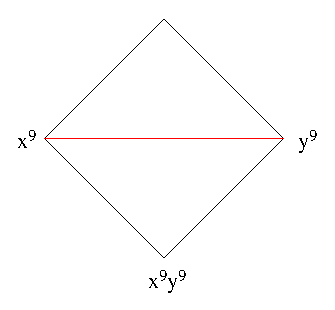
\includegraphics[width=2.5in]{TensorQuad5_Gauss}
%\caption{Pascal's triangle depiction of integrand monomial coverage 
%for two dimensions and Gaussian tensor-product quadrature order = 5.
%Red line depicts maximal total-order integrand coverage.}
%\label{fig:pascal_tensor_quad5_Gauss}
%\end{center}
%\end{figure} 

In~\cite{Eld09a}, it is demonstrated that close synchronization of
expansion form with the monomial resolution of a particular numerical
integration technique can result in significant performance
improvements.  In particular, the traditional approach of exploying a
total-order PCE (Eqs.~\ref{eq:to_multi_index}--\ref{eq:num_to_terms})
neglects a significant portion of the monomial coverage for a
tensor-product quadrature approach, and one should rather employ a
tensor-product PCE (Eqs.~\ref{eq:tp_multi_index}--\ref{eq:num_tp_terms}) 
to provide improved synchronization and more effective usage of the
Gauss point evaluations.  When the quadrature points are standard
Gauss rules (i.e., no Clenshaw-Curtis, Gauss-Patterson, or
Genz-Keister nested rules), it has been shown that tensor-product PCE
and SC result in identical polynomial forms~\cite{ConstTPQ},
completely eliminating a performance gap that exists between
total-order PCE and SC~\cite{Eld09a}.


\subsection{Smolyak sparse grids} \label{uq:expansion:spectral_sparse}

% For m = max points per dim, w = level:
%   Gaussian Smolyak: m = 2^(w+1) - 1  -->  m = 1, 3, 7, 15, 31, 63, 127
%   Clenshaw-Curtis:  m = 2^w     + 1  -->  m = 1, 3, 5,  9, 17, 33,  65
% TP logic would use:
%   Gaussian Smolyak: 2p <= 2m-1
%   Clenshaw-Curtis:  2p <=  m+1
% SG order selection instead using 2p <= m,
% as this is what has been observed thus far.

If the number of random variables is moderately large, one should rather
consider sparse tensor product spaces as first proposed by Smolyak
\cite{Smolyak_63} and further investigated by Refs.~\cite{gerstner_griebel_98,barth_novak_ritter_00,Fran_Schwab_Todor_04,Xiu_Hesthaven_05, webster1, webster2}
that reduce dramatically the number of collocation points, while
preserving a high level of accuracy.

Here we follow the notation and extend the description in
Ref.~\cite{webster1} to describe the Smolyak {\it isotropic} formulas
$\mathscr{A}({\rm w},n)$, where ${\rm w}$ is a level that is independent of
dimension\footnote{Other common formulations use a dimension-dependent
level $q$ where $q \geq n$.  We use $w = q - n$, where $w \geq 0$ for
all $n$.}.  The Smolyak formulas are just linear combinations of the
product formulas in Eq.~\ref{eq:multi_tensor} with the following key
property: only products with a relatively small number of points are
used.  With $\mathscr{U}^0 = 0$ and for $i \geq 1$ define
%
\begin{equation}\label{eq:delta}
\Delta^i = \mathscr{U}^i-\mathscr{U}^{i-1}.
\end{equation}
%

and we set $|\mathbf{i}| = i_1+\cdots + i_n$.
Then the isotropic Smolyak quadrature formula is given by
%
\begin{equation}\label{eq:smolyak1}
\mathscr{A}({\rm w},n) = \sum_{|\mathbf{i}| \leq {\rm w}+n}\left(\Delta^{i_1}\otimes\cdots\otimes\Delta^{i_n}\right).
\end{equation}
%
This form is preferred for use in forming hierarchical interpolants
as described in Sections~\ref{uq:expansion:interp:hierarch} 
and~\ref{uq:expansion:sc:hierarch}.  For nodal interpolants and 
polynomial chaos in sparse grids, the following equivalent 
form~\cite{was_woz} is often more convenient since it collapses 
repeated index sets
%
\begin{equation}\label{eq:smolyak2}
\mathscr{A}({\rm w},n) = \sum_{{\rm w}+1 \leq |\mathbf{i}| \leq {\rm w}+n}(-1)^{{\rm w}+n-|\mathbf{i}|}
{n-1 \choose {\rm w}+n-|\mathbf{i}|}\cdot
\left(\mathscr{U}^{i_1}\otimes\cdots\otimes\mathscr{U}^{i_n}\right).
\end{equation}

For each index set $\mathbf{i}$ of levels, linear or nonlinear growth
rules are used to define the corresponding one-dimensional quadrature
orders.  The following growth rules are employed for indices $i \geq
1$, where closed and open refer to the inclusion and exclusion of the
bounds within an interval, respectively:
% The following is more precisely presented by replacing w with i-1
%\begin{eqnarray}
%{\rm Clenshaw-Curtis:}~~m &=& 
%\left\{ \begin{array}{ll}
%         1       & w=0 \\
%         2^w + 1 & w \geq 1 
%        \end{array} \right.        \label{eq:growth_CC_nonlin} \\
%{\rm Gaussian:}~~m &=& 2^{w+1} - 1 \label{eq:growth_Gauss_nonlin}
%\end{eqnarray}
\begin{eqnarray}
{\rm closed~nonlinear:}~~m &=& 
\left\{ \begin{array}{ll}
         1       & i=1 \\
         2^{i-1} + 1 & i > 1 
        \end{array} \right.    \label{eq:growth_CC_nonlin} \\
{\rm open~nonlinear:}~~m &=& 2^i - 1 \label{eq:growth_Gauss_nonlin} \\
{\rm open~linear:}   ~~m &=& 2 i - 1 \label{eq:growth_Gauss_lin}
\end{eqnarray}
Nonlinear growth rules are used for fully nested rules (e.g.,
Clenshaw-Curtis is closed fully nested and Gauss-Patterson is open
fully nested), and linear growth rules are best for standard Gauss
rules that take advantage of, at most, ``weak'' nesting (e.g., reuse
of the center point).
%For fully nested quadrature rules such as Clenshaw-Curtis and
%%Gauss-Patterson, nonlinear growth rules are strongly preferred
%(Eq.~\ref{eq:growth_CC_nonlin} for the former and
%Eq.~\ref{eq:growth_Gauss_nonlin} for the latter).  For at most weakly
%nested Gaussian quadrature rules, either linear or nonlinear rules may
%be selected, with the former motivated by finer granularity of control
%and uniform integrand coverage and the latter motivated by consistency
%with Clenshaw-Curtis and Gauss-Patterson.  The $m = 2i - 1$ linear
%rule takes advantage of weak nesting (e.g., Gauss-Hermite and
%Gauss-Legendre), whereas non-nested rules (e.g., Gauss-Laguerre) could
%alternatively employ an $m = i$ linear rule without any loss of reuse.
%In the experiments to follow, Clenshaw-Curtis employs nonlinear growth
%via Eq.~\ref{eq:growth_CC_nonlin}, and all Gaussian rules employ
%either nonlinear growth from Eq.~\ref{eq:growth_Gauss_nonlin} or
%linear growth from Eq.~\ref{eq:growth_Gauss_lin}.

Examples of isotropic sparse grids, constructed from the fully nested 
Clenshaw-Curtis abscissas %described in Section \ref{sub:cc}, 
and the weakly-nested Gaussian abscissas %in Section \ref{sub:cc_gauss}, 
are shown in Figure \ref{fig:isogrid_N2_q7}, where $\Omega=[-1,1]^2$
and both Clenshaw-Curtis and Gauss-Legendre employ nonlinear
growth\footnote{We prefer linear growth for Gauss-Legendre, but employ
nonlinear growth here for purposes of comparison.} from
Eqs.~\ref{eq:growth_CC_nonlin} and~\ref{eq:growth_Gauss_nonlin},
respectively.  There, we consider a two-dimensional parameter space
and a maximum level ${\rm w}=5$ (sparse grid $\mathscr{A}(5,2)$).  To
see the reduction in function evaluations with respect to full tensor
product grids, we also include a plot of the corresponding
Clenshaw-Curtis isotropic full tensor grid having the same maximum
number of points in each direction, namely $2^{\rm w}+1 = 33$.
%Whereas an isotropic tensor-product quadrature scales as $m^n$, an
%isotropic sparse grid scales as $m^{{\rm log}~n}$, significantly
%mitigating the curse of dimensionality.
%
\begin{figure}[h!]
%\vspace{-2cm}
\begin{center}
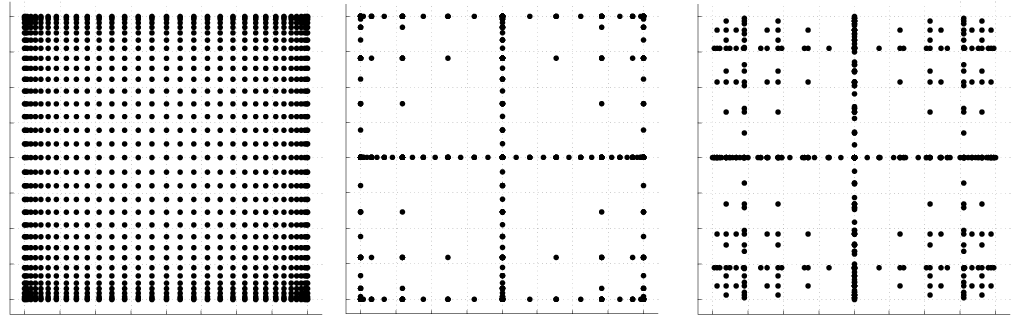
\includegraphics[width=6.5in]{images/isogrid_N2_q6}
\caption{Two-dimensional grid comparison with a tensor product grid
  using Clenshaw-Curtis points (left) and sparse grids
  $\mathscr{A}(5,2)$ utilizing Clenshaw-Curtis (middle) and
  Gauss-Legendre (right) points with nonlinear growth. }
\label{fig:isogrid_N2_q7}
\end{center}
\end{figure}

%Figure~\ref{fig:pascal_sparse_lev4_Gauss} depicts the monomial
%coverage in Pascal's triangle for two-dimensional level 4 isotropic
%sparse grids ($\mathscr{A}(4,2)$) employing the same one-dimensional
%Gaussian integration rule, where
%Figure~\ref{fig:pascal_sparse_lev4_Gauss}(a) shows the application of
%a nonlinear growth rule as given in Eq.~\ref{eq:growth_Gauss_nonlin}
%and Figure~\ref{fig:pascal_sparse_lev4_Gauss}(b) shows the use of a
%linear growth rule as given in Eq.~\ref{eq:growth_Gauss_lin}.  Using
%this geometric interpretation, subtracted tensor-product grids from
%Eqs.~\ref{eq:delta} and \ref{eq:smolyak2} can be interpreted as
%regions of overlap where only a single contribution to the integral
%should be retained.  And for these monomial coverage patterns, the
%traditional approach of exploying a total-order PCE (maximal
%resolvable total-order integrand depicted with red horizontal line)
%can be seen to be well synchronized for the case of linear growth
%rules (since only a few small ``teeth'' protrude beyond the maximal
%total-order basis) and to be somewhat conservative for nonlinear
%growth rules due to the ``hyperbolic cross'' shape (since the maximal
%total-order basis is dictated by the concave interior, neglecting the
%extended coverage along the axes).
%
%However, the inclusion of additional terms beyond the
%total-order basis in the nonlinear growth rule case, as motivated by
%the legs in Figure~\ref{fig:pascal_sparse_lev4_Gauss}(a), would be
%error-prone, since the order of the unknown response function will
%tend to push the product integrand (Eq.~\ref{eq:coeff_extract}) out
%into the concave interior, resulting in product polynomials that are
%not resolvable by the sparse integration.
%\begin{figure}[htbp]
%  \begin{subfigmatrix}{2}
%  \subfigure[Nonlinear growth rule.]{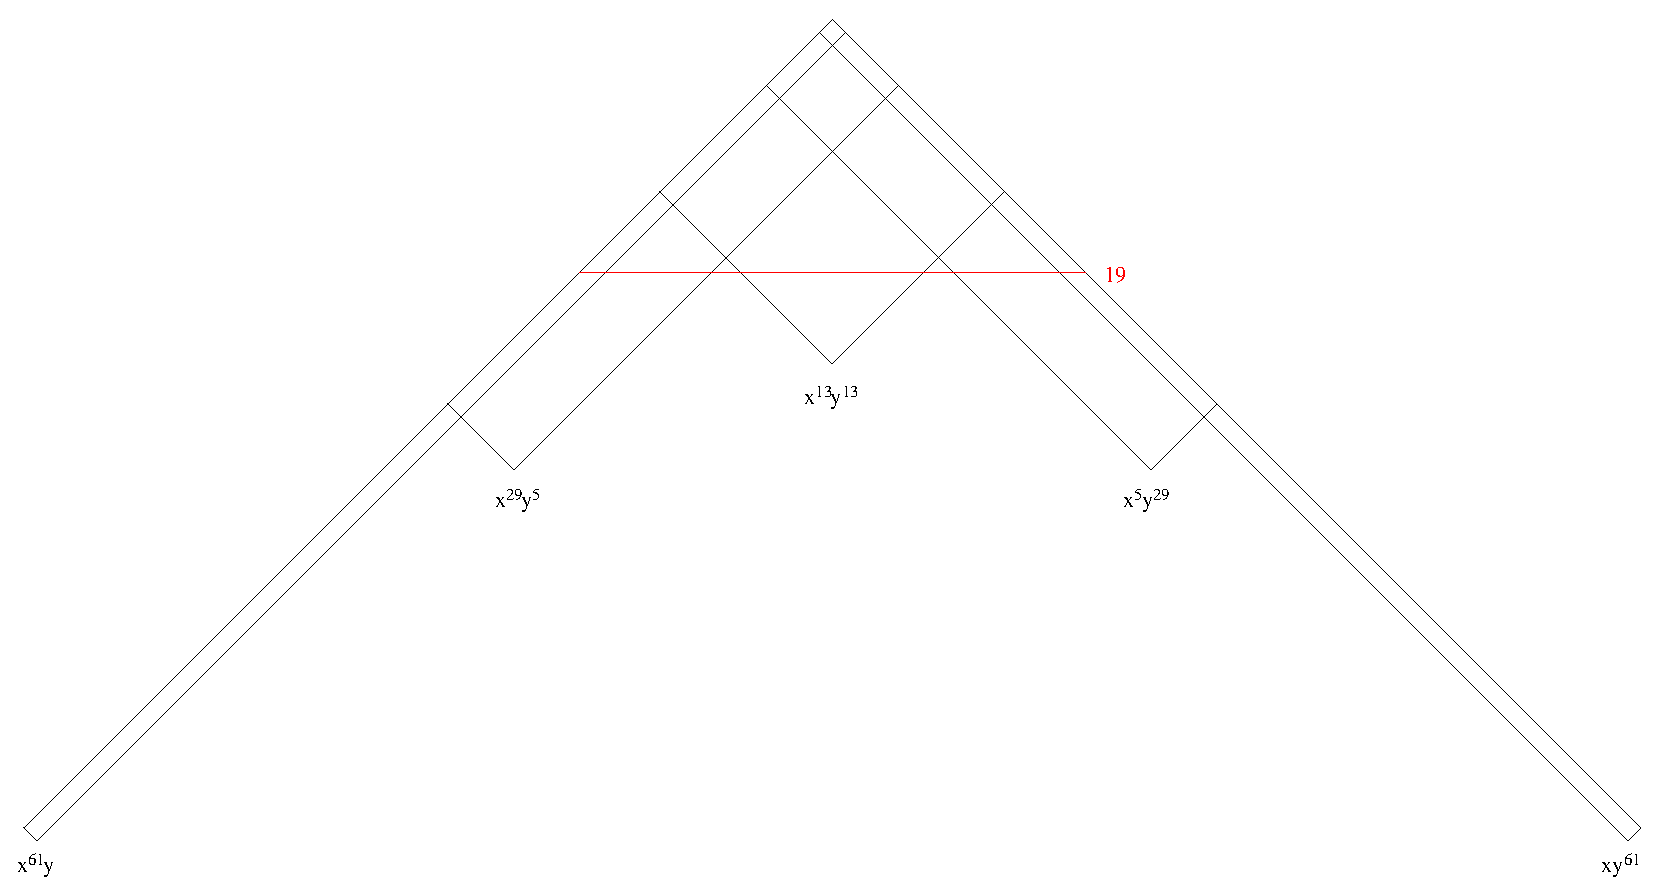
\includegraphics{SparseLevel4_NonlinGauss}}
%  \subfigure[Linear growth rule.]{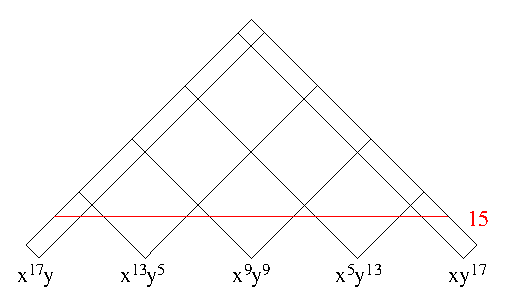
\includegraphics{SparseLevel4_LinGauss}}
%  \end{subfigmatrix}
%  \caption{Pascal's triangle depiction of integrand monomial coverage 
%for two dimensions and Gaussian sparse grid level = 4.  Red line depicts 
%maximal total-order integrand coverage.}
%\label{fig:pascal_sparse_lev4_Gauss}
%\end{figure}
%For the total-order PCE basis, the integrand monomial coverage must
%again resolve $2p$, such that $p = 9$ would be selected in this
%nonlinear growth rule example and $p = 7$ would be selected in the
%linear growth rule example.

In~\cite{Eld09a}, it is demonstrated that the synchronization of
total-order PCE with the monomial resolution of a sparse grid is
imperfect, and that sparse grid SC consistently outperforms sparse
grid PCE when employing the sparse grid to directly evaluate the
integrals in Eq.~\ref{eq:coeff_extract}.  In our Dakota implementation, we 
depart from the use of sparse integration of total-order expansions, and 
instead employ a linear combination of tensor expansions~\cite{ConstSSG}.
%That is, instead of employing the sparse grid as a separate numerical
%integration scheme for evaluations of Eq.~\ref{eq:coeff_extract} (for 
%which expansion synchronization is a challenge), we instead 
That is, we compute separate tensor polynomial chaos expansions for
each of the underlying tensor quadrature grids (for which there is no
synchronization issue) and then sum them using the Smolyak
combinatorial coefficient (from Eq.~\ref{eq:smolyak2} in the isotropic
case).  This improves accuracy, preserves the PCE/SC consistency
property described in Section~\ref{uq:expansion:spectral_quad}, and also
simplifies PCE for the case of anisotropic sparse grids described next.

For anisotropic Smolyak sparse grids, a dimension preference vector is
used to emphasize important stochastic dimensions.  
%A natural mechanism for quantifying
%dimension importance is through the global sensitivity analysis
%procedure described in Section~\ref{sec:ssa:global}, as the
%attribution of output variance among input sources provides an
%intuitive measure of importance in the stochastic setting.
Given a mechanism for defining anisotropy, we can extend the
definition of the sparse grid from that of Eq.~\ref{eq:smolyak2} to
weight the contributions of different index set components.  First,
the sparse grid index set constraint becomes
\begin{equation}
{\rm w}\underline{\gamma} < \mathbf{i} \cdot \mathbf{\gamma} \leq 
{\rm w}\underline{\gamma}+|\mathbf{\gamma}|
\label{eq:aniso_smolyak_constr}
\end{equation}
where $\underline{\gamma}$ is the minimum of the dimension weights
$\gamma_k$, $k$ = 1 to $n$.  The dimension weighting vector
$\mathbf{\gamma}$ amplifies the contribution of a particular dimension
index within the constraint, and is therefore inversely related to the
dimension preference (higher weighting produces lower index set
levels).  For the isotropic case of all $\gamma_k = 1$, it is evident
that you reproduce the isotropic index constraint ${\rm w}+1 \leq
|\mathbf{i}| \leq {\rm w}+n$ (note the change from $<$ to $\leq$).
Second, the combinatorial coefficient for adding the contribution from
each of these index sets is modified as described in~\cite{Burk09}.
%Given the modified index sets and combinatorial coefficients defined
%from the dimension preference vector, interpolation (SC) on
%anisotropic sparse grids proceeds as for the isotropic case.  PCE,
%however, again has the challenge of expansion tailoring.  Fortunately,
%in the anistropic case, we can assume that more is known about the
%form of the response function (especially if the dimension preference
%was based on variance-based decomposition).  This allows us to abandon
%the safe total-order basis approach in favor of a tightly-synchronized
%expansion formulation that applies the $2p$ logic to all of the
%protruding ``legs'' in the monomial resolution structure.


\subsection{Cubature} \label{uq:expansion:cubature}

Cubature rules~\cite{stroud,xiu_cubature} are specifically optimized
for multidimensional integration and are distinct from tensor-products 
and sparse grids in that they are not based on combinations of 
one-dimensional Gauss quadrature rules.  They have the advantage of 
improved scalability to large numbers of random variables, but are 
restricted in integrand order and require homogeneous random variable 
sets (achieved via transformation).  For example, optimal rules for
integrands of 2, 3, and 5 and either Gaussian or uniform densities 
allow low-order polynomial chaos expansions ($p=1$ or $2$) that are 
useful for global sensitivity analysis including main effects and, 
for $p=2$, all two-way interactions.


\section{Linear regression} \label{uq:expansion:regress}

Regression based approaches attempt to find regularized or exact
solutions of the linear system:
\begin{equation}
\boldsymbol{\Psi} \boldsymbol{\alpha} = \boldsymbol{R} \label{eq:regression}
\end{equation}
to solve for the complete set of PCE coefficients
$\boldsymbol{\alpha}$ that best reproduce a set of response values
$\boldsymbol{R}$.  The set of response values can be defined on an
unstructured grid obtained from sampling within the density function
of $\boldsymbol{\xi}$ (point collocation~\cite{pt_colloc1,pt_colloc2})
or on a structured grid defined from uniform random sampling on the
multi-index\footnote{Due to the discrete nature of index sampling, we
  enforce unique index samples by sorting and resampling as required.}
of a tensor-product quadrature grid (probabilistic
collocation~\cite{Tat95}), where the quadrature is of sufficient order
to avoid sampling at roots of the basis polynomials\footnote{Generally
  speaking, dimension quadrature order $m_i$ greater than dimension
  expansion order $p_i$.}.  In either case, each row of the matrix
$\boldsymbol{\Psi}$ contains the $N_t$ multivariate polynomial terms
$\Psi_j$ evaluated at a particular $\boldsymbol{\xi}$ sample.  An
over-sampling is most commonly used (\cite{pt_colloc2} recommends
$2N_t$ samples), resulting in a least squares solution for the
over-determined system, although unique determination ($N_t$ samples)
and under-determination (fewer than $N_t$ samples) are also supported.
As for sampling-based coefficient estimation, this approach is only
valid for PCE and does not require synchronization with monomial
coverage; thus it is common to combine this coefficient estimation
approach with a traditional total-order chaos expansion in order to
keep sampling requirements low.  In this case, simulation requirements
for this approach scale as $\frac{r(n+p)!}{n!p!}$ ($r$ is an
over-sampling factor with typical values $0.1 \leq r \leq 2$), which
can be significantly more affordable than isotropic tensor-product
quadrature (scales as $(p+1)^n$ for standard Gauss rules) for larger
problems.
%A closely related technique is known as the ``probabilistic
%collocation'' approach.  Rather than employing random over-sampling,
%this technique uses a selected subset of $N_t$ Gaussian quadrature
%points (those with highest tensor-product weighting), which provides
%more optimal collocation locations and preserves interpolation
%properties.
Additional regression equations can be obtained through the use of
derivative information (gradients and Hessians) from each collocation
point (refer to {\tt use\_derivatives} in the PCE regression
specification details in the Dakota Reference Manual~\cite{RefMan}),
which can aid in scaling with respect to the number of random
variables, particularly for adjoint-based derivative approaches.
Finally, one can additionally modify the order of the exponent 
applied to $N_t$ in the over-sampling ratio calculation (refer to 
{\tt ratio\_order} in the PCE regression specification details in the
Dakota Reference Manual~\cite{RefMan}).

Various methods can be employed to solve \eqref{eq:regression}.  The
relative accuracy of each method is problem dependent. Traditionally,
the most frequently used method has been least squares
regression. However when $\boldsymbol{\Psi}$ is under-determined,
minimizing the residual with respect to the $\ell_2$ norm typically
produces poor solutions. Compressed sensing methods have been
successfully used to address this
limitation~\cite{Blatman2011,Doostan2011}.  Such methods attempt to
only identify the elements of the coefficient vector
$\boldsymbol{\alpha}$ with the largest magnitude and enforce as many
elements as possible to be zero. Such solutions are often called
sparse solutions. Dakota provides algorithms that solve the following
formulations:
\begin{itemize}
 \item Basis Pursuit (BP)~\cite{Chen2001}
\begin{equation}
\label{eq:bp}
\boldsymbol{\alpha} = \text{arg min} \; \|\boldsymbol{\alpha}\|_{\ell_1}\quad \text{such that}\quad \boldsymbol{\Psi}\boldsymbol{\alpha} = \boldsymbol{R}
\end{equation}
The BP solution is obtained in Dakota, by transforming~\eqref{eq:bp} to a 
linear program which is then solved using the primal-dual
interior-point method~\cite{Boyd2004,Chen2001}.
\item Basis Pursuit DeNoising (BPDN)~\cite{Chen2001}. 
\begin{equation}
\label{eq:bpdn}
\boldsymbol{\alpha} = \text{arg min}\; \|\boldsymbol{\alpha}\|_{\ell_1}\quad \text{such that}\quad \|\boldsymbol{\Psi}\boldsymbol{\alpha} - \boldsymbol{R}\|_{\ell_2} \le \varepsilon
\end{equation}
The BPDN solution is computed in Dakota by transforming~\eqref{eq:bpdn} 
to a quadratic cone problem which is solved using the log-barrier Newton 
method~\cite{Boyd2004,Chen2001}. 


When the matrix $\boldsymbol{\Psi}$ is not over-determined the BP and BPDN solvers used in Dakota
will not return a solution. In such situations these methods simply return the least squares solution.
\item Orthogonal Matching Pursuit (OMP)~\cite{Davis1997},
\begin{equation}
\label{eq:omp}
\boldsymbol{\alpha} = \text{arg min}\; \|\boldsymbol{\alpha}\|_{\ell_0}\quad \text{such that}\quad \|\boldsymbol{\Psi}\boldsymbol{\alpha} - \boldsymbol{R}\|_{\ell_2} \le \varepsilon
\end{equation}
OMP is a heuristic method which greedily finds an approximation to~\eqref{eq:omp}. In contrast to the aforementioned techniques for solving BP and BPDN, 
which minimize an objective function, OMP constructs a sparse solution by iteratively 
building up an approximation of the solution vector $\boldsymbol{\alpha}$. 
The vector is approximated as a linear combination of a subset of active columns of 
$\boldsymbol{\Psi}$. The active set of columns is built column by column, in
a greedy fashion, such that at each iteration the inactive column with the highest correlation
(inner product) with the current residual is added.

\item Least Angle Regression (LARS)~\cite{Efron2004} and Least Absolute Shrinkage and Selection Operator (LASSO)~\cite{Tibshirani1996}
\begin{equation}
\label{eq:lasso}
 \boldsymbol{\alpha} = \text{arg min}\; \|\boldsymbol{\Psi}\boldsymbol{\alpha} - \boldsymbol{R}\|_{\ell_2}^2 \quad \text{such that}\|\boldsymbol{\alpha}\|_{\ell_1} \le \tau
\end{equation}
A greedy solution can be found to~\eqref{eq:lasso} using the LARS algorithm.
Alternatively, with only a small modification, one can provide a rigorous solution to this global optimization problem, which we refer to as the LASSO solution. Such an approach is identical to the homotopy algorithm of
Osborne et al~\cite{Osborne2000}. It is interesting to note that 
Efron~\cite{Efron2004} experimentally observed that the basic, faster LARS 
procedure is often identical to the LASSO solution.

The LARS algorithm is similar to OMP. LARS again maintains an active set of columns and again builds
this set by adding the column with the largest correlation with the residual to the current residual.
However, unlike OMP, LARS solves a penalized least squares problem at each step taking a step along an equiangular direction, that is, a direction
having equal angles with the vectors in the active set. LARS and OMP do not allow a column (PCE basis)
to leave the active set. However if this restriction is removed from LARS (it cannot be from OMP)
the resulting algorithm can provably solve~\eqref{eq:lasso} and generates the LASSO solution.

\item Elastic net~\cite{Zou2005}
\begin{equation}
\label{eq:elastic-net}
 \boldsymbol{\alpha} = \text{arg min}\; \|\boldsymbol{\Psi}\boldsymbol{\alpha} - \boldsymbol{R}\|_{\ell_2}^2 \quad \text{such that}\quad (1-\lambda)\|\boldsymbol{\alpha}\|_{\ell_1} + 
\lambda\|\boldsymbol{\alpha}\|_{\ell_2}^2 \le \tau
\end{equation}
The elastic net was developed to overcome some of the limitations of the LASSO formulation. 
Specifically: if the ($M\times N$) Vandermonde matrix $\boldsymbol{\Psi}$ is over-determined ($M>N$), 
the LASSO selects at most $N$ variables before it saturates, because of the
nature of the convex optimization problem; if there is a group of variables among which the pairwise correlations are very high, then
the LASSO tends to select only one variable from the group and does not care which one is
selected; and finally if there are high correlations between predictors, it has been
empirically observed that the prediction performance of the LASSO is dominated by ridge
regression~\cite{Tibshirani1996}. Here we note that it is hard to estimate the $\lambda$ 
penalty in practice and the aforementioned issues typically do not arise very often when 
solving~\eqref{eq:regression}. The elastic net formulation can be solved with a minor modification of
the LARS algorithm.
\end{itemize}

\begin{figure}[h]
\centering
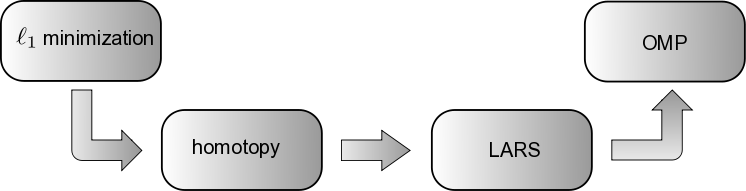
\includegraphics[width=0.95\textwidth]{images/compressed-sensing-hierarchy.png}
\caption{Bridging provably convergent $\ell_1$ minimization algorithms and greedy 
algorithms such as OMP. (1) Homotopy provably solves $\ell_1$ minimization 
problems~\cite{Efron2004}. (2) LARS is obtained from homotopy by removing
the sign constraint check. (3) OMP and LARS are similar in structure, 
the only difference being that OMP solves a least-squares problem at each iteration,
whereas LARS solves a linearly penalized least-squares problem. 
Figure and caption based upon Figure 1 in~\cite{Donoho2008}.}
\label{fig:compressed-sensing-method-heirarchy}
\end{figure}

OMP and LARS add a PCE basis one step at a time. If $\boldsymbol{\alpha}$ contains
 only $k$ non-zero terms then these methods will only take $k$-steps. 
The homotopy version of LARS also adds only basis at each step, however 
it can also remove bases, and thus can take more than $k$ steps. For some problems, 
the LARS and homotopy solutions will coincide. Each step of these algorithm provides a possible
estimation of the PCE coefficients. However, without knowledge of the target function, there is no
easy way to estimate which coefficient vector is best. With some additional computational 
effort (which will likely be minor to the cost of obtaining model simulations), cross validation 
can be used to choose an appropriate coefficient vector.

\subsection{Cross validation}

Cross validation can be used to find a coefficient vector $\boldsymbol{\alpha}$ 
that approximately minimizes $\| \hat{f}(\mathbf{x})-f(\mathbf{x})\|_{L^2(\rho)}$, where
$f$ is the target function and $\hat{f}$ is the PCE approximation using $\boldsymbol{\alpha}$. 
Given training data $\mathbf{X}$ and a set of algorithm parameters $\boldsymbol{\beta}$ (which can be step number in an 
algorithm such as OMP, or PCE maximum degree), $K$-folds cross validation divides 
$\mathbf{X}$ into $K$ sets (folds) $\mathbf{X}_k$, $k=1,\ldots,K$ of equal size. 
A PCE $\hat{f}^{-k}_{\boldsymbol{\beta}}(\mathbf{X})$, is built on the training data 
$\mathbf{X}_{\mathrm{tr}}=\mathbf{X} \setminus \mathbf{X}_k$ 
with the $k$-th fold removed, using the tuning parameters $\boldsymbol{\beta}$. 
The remaining data $\mathbf{X}_k$ is then used to estimate the prediction error.
The prediction error is typically approximated by
$e(\hat{f})=\lVert \hat{f}(\mathbf{x})-f(\mathbf{x})\rVert_{\ell_2}$, 
$\mathbf{x}\in\mathbf{X}_{k}$~\cite{hastie2001}. This process is then repeated $K$ times, removing a 
different fold from the training set each time. 

The cross validation error is taken to be the average of the prediction errors for the $K$-experiments
\[
CV(\hat{f}_{\boldsymbol{\beta}}) = \mathrm{E}[e(\hat{f}_{\boldsymbol{\beta}}^{-k})] = \frac{1}{K}\sum_{k=1}^K e(\hat{f}_{\boldsymbol{\beta}}^{-k})
\]
We minimize $CV(\hat{f}_{\boldsymbol{\beta}})$ as a surrogate for minimizing
$\| \hat{f}_{\boldsymbol{\beta}}(\mathbf{x})-f(\mathbf{x})\|_{L^2(\rho)}$ and choose the tuning parameters 
\begin{equation}
\label{eq:optimal_tuning-parameters}
\boldsymbol{\beta}^\star = \text{arg min}\, CV(\hat{f}_{\boldsymbol{\beta}})\mathrm{Var}[e(\hat{f}_{\boldsymbol{\beta}}^{-k})]
\end{equation}
to construct the final ``best'' PCE approximation of $f$ that the training data can produce. 
\subsection{Iterative basis selection}
\label{sec:iterative-basis-selection}
When the coefficients of a PCE can be well approximated by a sparse vector, $\ell_1$-minimization is extremely effective at recovering the coefficients of that PCE. 
It is possible, however, to further increase the efficacy of $\ell_1$-minimization by leveraging realistic models of structural dependencies between the values and 
locations of the PCE coefficients. For example~\cite{Baraniuk_CDH_IEEIT_2010,Duarte_WB_SPARS_2005,La_D_IEEEIP_2006} have successfully increased the performance
of $\ell_1$-minimization when recovering wavelet coefficients that exhibit a tree-like structure. In this vein, we propose an algorithm for identifying the large coefficients
of PC expansions that form a semi-connected subtree of the PCE coefficient tree.

The coefficients of polynomial chaos expansions often form a multi-dimensional tree.
Given an ancestor basis term $\phi_{\boldsymbol{\lambda}}$ of degree $\left\lVert \boldsymbol{\lambda} \right\rVert_{1}$ we define the indices of its children as $\boldsymbol{\lambda}+\mathbf{e}_k$, $k=1,\ldots,d$,
where $\mathbf{e}_k=(0,\ldots,1,\ldots,0)$ is the unit vector co-directional with the $k$-th dimension.
% We refer to the basis terms with $\hat{\boldsymbol{\lambda}}-\be_k$ as ancestors of the basis indexed by $\hat{\boldsymbol{\lambda}}$.
An example of a typical PCE tree is depicted in Figure~\ref{fig:pce-tree}. In this figure, as often in practice, the magnitude of the ancestors of a PCE coefficient is a
reasonable indicator of the size of the child coefficient. In practice, some branches (connections) between levels of the tree may be missing. We refer to trees with missing branches 
as semi-connected trees.

In the following we present a method for estimating PCE coefficients that leverages the tree structure of 
PCE coefficients to increase the accuracy of coefficient estimates obtained by $\ell_1$-minimization.
\begin{figure}
\centering
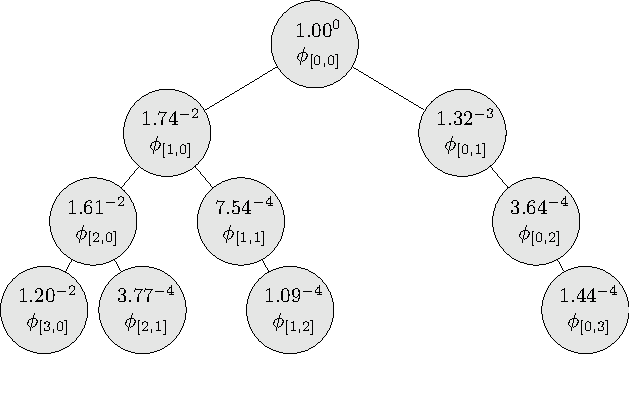
\includegraphics[width=0.75\textwidth]{images/pce-tree.pdf}
\caption{Tree structure of the coefficients of a two dimensional PCE with a total-degree basis of order 3. For clarity we only depict one connection per node, but in $d$ dimensions a node of a given
degree $p$ will be a child of up to $d$ nodes of degree $p-1$. For example, not only is the basis $\boldsymbol{\phi}_{[1,1]}$ a child of $\boldsymbol{\phi}_{[1,0]}$ (as depicted) but it is
 also a child of $\boldsymbol{\phi}_{[0,1]}$} 
\label{fig:pce-tree}
\end{figure}

Typically $\ell_1$-minimization is applied to an a priori chosen and fixed basis set $\Lambda$. However the accuracy of coefficients obtained by $\ell_1$-minimization can be increased by
adaptively selecting the PCE basis.

To select a basis for $\ell_1$-minimization we employ a four step iterative procedure involving restriction, expansion, identification and selection. 
The iterative basis selection procedure is outlined in Algorithm~\ref{alg:basis-selection}. A graphical version of the algorithm is also presented in Figure~\ref{fig:basis-selection-alg}.
The latter emphasizes the four stages of basis selection, that is restriction, growth, identification and selection. These four stages are also highlighted in 
Algorithm~\ref{alg:basis-selection} using the corresponding colors in Figure~\ref{fig:basis-selection-alg}.

To initiate the basis selection algorithm, we first define a basis set $\Lambda^{(0)}$ and use $\ell_1$-minimization to identify the largest coefficients $\boldsymbol{\alpha}^{(0)}$. The choice of $\Lambda^{(0)}$
can sometimes affect the performance of the basis selection algorithm. We found a good choice to be $\Lambda^{(0)}=\Lambda_{p,1}$,
where $p$ is the degree that gives $\lvert\Lambda^d_{p,1}\rvert$ closest to $10M$, i.e. $\Lambda^d_{p,1} = \argmin_{\Lambda^d_{p,1}\in\{\Lambda^d_{1,1},\Lambda^d_{2,1},\ldots\}}\abs{\lvert\Lambda^d_{p,1}\rvert-10M}$.
Given a basis $\Lambda^{(k)}$ and corresponding coefficients $\boldsymbol{\alpha}^{(k)}$ we reduce the basis to a set $\Lambda^{(k)}_\varepsilon$ containing only the terms with non-zero coefficients. 
This restricted basis is then expanded $T$ times using an algorithm which we will describe in Section~\ref{sec:basisexp}. $\ell_1$-minimization is then applied to each of the expanded basis 
sets $\Lambda^{(k,t)}$ for $t=1,\dots, T$.
Each time $\ell_1$-minimization is used, we employ cross validation to choose $\varepsilon$. Therefore, at every basis set considered during the evolution of the algorithm we have a measure
of the expected accuracy of the PCE coefficients. At each step in the algorithm we choose the basis set that results in the lowest cross validation~error.


\begin{algorithm}[H]
%\dontprintsemicolon%
\DontPrintSemicolon % Some LaTeX compilers require you to use \dontprintsemicolon instead
\footnotesize
$\Lambda^{\star} = \Lambda^{(0)} = \Lambda^d_{p,1} = \argmin_{\Lambda^d_{p,1}\in\{\Lambda^d_{1,1},\Lambda^d_{2,1},\ldots\}}\abs{\card{\Lambda^d_{p,1}}-10M}$\;
$\boldsymbol{\alpha}^{(0)}$, $e_{\mathrm{cv}}^{(0)}$ = $\ell_1$-minimization[$\boldsymbol{\phi}(\Lambda^{(0)})$,$\mathbf{f}$]\;
$T=3$, $e_{\mathrm{cv}}^\star = \infty$, $k = 1$\;
\While{TRUE}{
  $e_{\mathrm{cv}}^{(k)}=\infty$\;
  \RHiLi$\Lambda^{(k,0)}=\{\boldsymbol{\lambda}:\boldsymbol{\lambda}\in\Lambda^{(k-1)}, \boldsymbol{\alpha}_{\boldsymbol{\lambda}}^{(k)} \ne 0\}$\;
  \For{$t\in\{1,\ldots,T\}$}{
     \EHiLi$\Lambda^{(k,t)}$ = EXPAND[$\Lambda^{(k,t-1)}$]\;
     \IHiLi$\boldsymbol{\alpha}^{(k,t)}$, $e_{\mathrm{cv}}^{(k,t)}$ = $\ell_1$-minimization[$\boldsymbol{\phi}(\Lambda^{(k,t)})$,$\mathbf{f}$]\;
     \If {$e_{\mathrm{cv}}^{(k,t)}<e_{\mathrm{cv}}^{(k)}$} {\SHiLi$e_{\mathrm{cv}}^{(k)}=e_{\mathrm{cv}}^{(k,t)}$, $\boldsymbol{\alpha}^{(k)}=\boldsymbol{\alpha}^{(k,t)}$, $\Lambda^{(k)}=\Lambda^{(k,t)}$}
 }
  \If{$e_{\mathrm{cv}}^{(k)} > e_{\mathrm{cv}}^\star$}{ TERMINATE }
  $\alpha^\star=\boldsymbol{\alpha}^{(k)},\; \Lambda^\star=\Lambda^{(k)},\; e_{\mathrm{cv}}^\star=e_{\mathrm{cv}}^{(k)}$\;%, $\Lambda^\star=\{\boldsymbol{\lambda}:\boldsymbol{\lambda}\in\Lambda^{(k)}, \boldsymbol{\alpha}_{\boldsymbol{\lambda}} \ne 0\}$, $\boldsymbol{\alpha}^\star = \{\boldsymbol{\alpha}_{\boldsymbol{\lambda}} : \boldsymbol{\lambda}\in\Lambda^{(k)} ,\boldsymbol{\alpha}_{\boldsymbol{\lambda}}\ne 0\}$\;
%   $k=k+1$\;
}
\caption{$\Lambda^\star$,$\boldsymbol{\alpha}^\star$=BASIS\_SELECTION[$\boldsymbol{\phi}$,$\mathbf{f}$,$\varepsilon$] }
\label{alg:basis-selection}
\end{algorithm}

\begin{figure}
%\includegraphics[width=1\textwidth]{basis-adaptation-algorithm-summary}
\hspace{-2cm}\includegraphics[width=1.3\textwidth]{images/basis-adaptation-algorithm-summary}
\caption{Graphical depiction of the basis adaptation algorithm.}
\label{fig:basis-selection-alg}
\end{figure}
\subsubsection{Basis expansion} \label{sec:basisexp}

Define $\{\boldsymbol{\lambda}+\mathbf{e}_j:1\le j\le d\}$ the forward neighborhood of an index $\boldsymbol{\lambda}$ and similarly let $\{\boldsymbol{\lambda}-\mathbf{e}_j:1\le j\le d\}$ denote the backward neighborhood.
To expand a basis set $\Lambda$ we must first find the forward neighbors $\mathcal{F}=\{\boldsymbol{\lambda}+\mathbf{e}_j : \boldsymbol{\lambda}\in\Lambda, 1\le j\le d \}$ of all indices $\boldsymbol{\lambda}\in\Lambda$.
The expanded basis is then given by 
\[
\Lambda^+=\Lambda\cup\mathcal{A},\quad \mathcal{A}=\{\boldsymbol{\lambda}: \boldsymbol{\lambda}\in\mathcal{F}, \boldsymbol{\lambda}-\mathbf{e}_n\in\Lambda\text{ for }1\le n\le d,\, \lambda_k > 1\}
\]
where we have used the following admissibility criteria 
\begin{equation}
\label{eq:admissibility}
\boldsymbol{\lambda}-\mathbf{e}_n\in\Lambda\text{ for }1\le n\le d,\, \lambda_k > 1
\end{equation}
to target PCE basis indices that are likely to have large PCE coefficients. A forward neighbor is admissible only if its backward neighbors exist in all dimensions. 
If the backward neighbors do not exist then $\ell_1$-minimization has previously identified that the coefficients of these backward neighbors are negligible. 

The admissibility criterion is explained graphically in Figure~\ref{fig:index-dmissibiliy-examples}. In the left graphic, 
both children of the current index are admissible, because its backwards neighbors exist in every dimension. 
In the right graphic only the child in the vertical dimension is admissible,
as not all parents of the horizontal child exist. 
\begin{figure}[ht]
\begin{center}
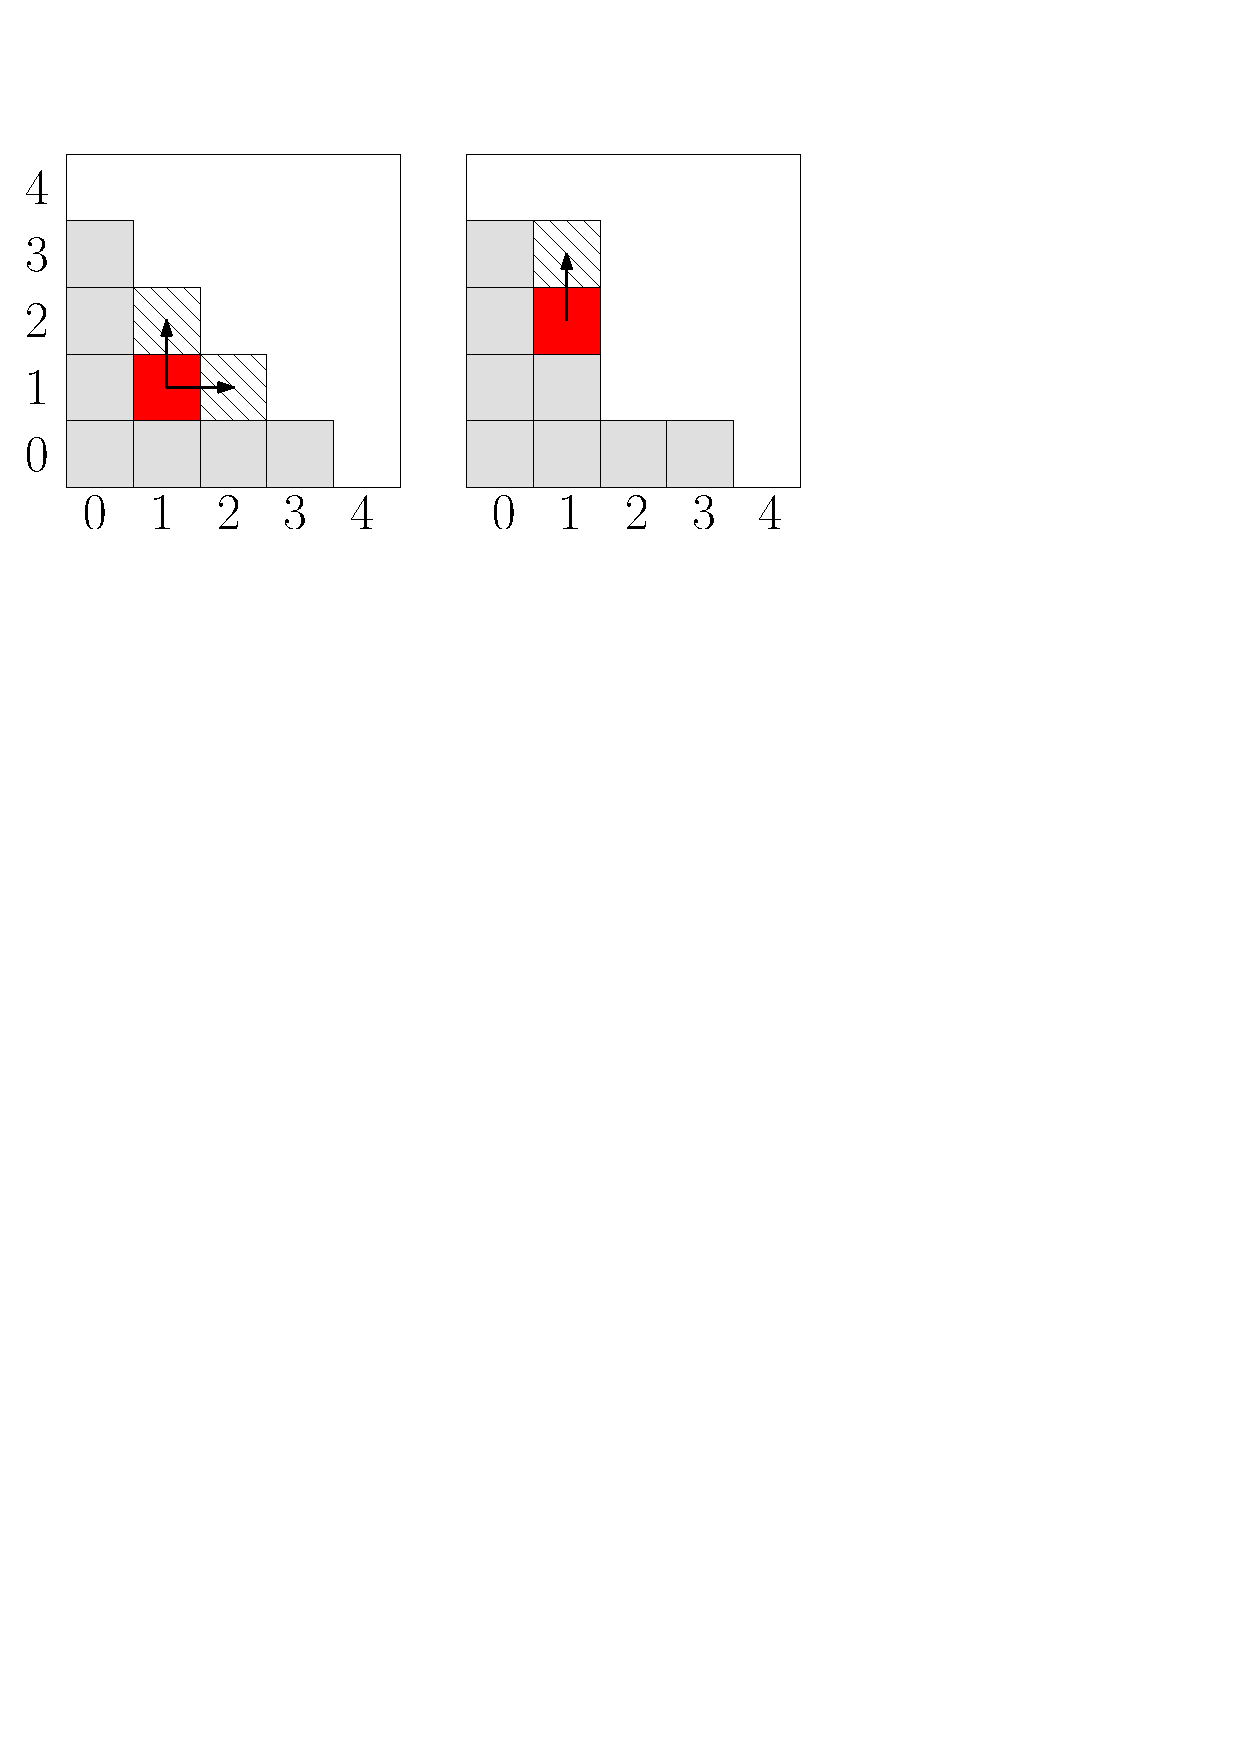
\includegraphics[width=0.95\textwidth]{images/index-expansion}
\caption{Identification of the admissible indices of an index (red). The indices of the current basis $\Lambda$ are gray and admissible indices are striped. A index is admissible only if
its backwards neighbors exists in every dimension.}
\label{fig:index-dmissibiliy-examples}
\end{center}
\end{figure}

At the $k$-th iteration of Algorithm~\ref{alg:basis-selection}, $\ell_1$-minimization is applied to $\Lambda^{(k-1)}$ and used to identify the significant coefficients of the PCE and their corresponding basis terms $\Lambda^{(k,0)}$. 
The set of non-zero coefficients $\Lambda^{(k,0)}$ identified by $\ell_1$-minimization is then expanded. 
% The key to the proposed method working well is to ensure the basis generated by expansion is able capture higher degree terms without increasing the mutual coherence
% to a point which degrades the ability of $\ell_1$-minimization to recover those higher order terms. 
The \texttt{EXPAND} routine expands an index set by one polynomial degree,
but sometimes it may be necessary to expand the basis $\Lambda^{(k)}$ more than once.\footnote{The choice of $T>1$ enables the basis selection algorithm to be applied to semi-connected 
tree structures as well as fully connected trees. Setting $T>1$ allows us to prevent premature termination of
the algorithm if most of the coefficients of the children of the current set $\Lambda^{(k)}$ are small but the coefficients of the children's children are not.}
%For example by more than one degree to avoid situations when no basis terms one degree higher are significant, but basis terms two or three degrees higher are. 
To generate these higher degree index sets \texttt{EXPAND} is applied recursively to $\Lambda^{(k,0)}$ up to a fixed number of $T$ times.
Specifically, the following sets are generated
$$\Lambda^{(k,t)}=\Lambda^{(k,t-1)}\cup\{\boldsymbol{\lambda}:\boldsymbol{\lambda}-\mathbf{e}_n\in\Lambda^{(k,t-1)},1\le n\le d,\, \lambda_n > 1\}.$$  
As the number of expansion steps $T$ increases the number of terms in the expanded basis increases rapidly and
degradation in the performance of $\ell_1$-minimization can result (this is similar to what happens when increasing the degree of a total degree basis). 
To avoid degradation of the solution, we use cross validation to choose the number of inner expansion steps $t\in[1,T]$.

\subsection{Orthogonal Least Interpolation}
Orthogonal least interpolation (OLI)~\cite{narayan12} enables the construction of  interpolation polynomials based on arbitrarily located grids in arbitrary dimensions. The interpolation polynomials can be constructed using using orthogonal polynomials corresponding to the probability distribution function of the uncertain random variables. 

The algorithm for constructing an OLI is split into three stages: 
(i) basis determination - transform the orthogonal basis into a polynomial space
that is “amenable” for interpolation;
(ii) coefficient determination - determine the interpolatory coefficients on the transformed basis elements;
(iii) connection problem - translate the coefficients on the transformed basis to coefficients in the original orthogonal basis
These three steps can be achieved by a sequence of LU and QR factorizations.

Orthogonal least interpolation is closesly related to the aforementioned regression methods, in that OLI can be used to build approximations of simulation models when computing structured simulation data, such as sparse grids or cubature nodes, is infeasiable. The interpolants produced by OLI have two additional important properties. Firstly, the orthogonal least interpolant is the lowest-degree polynomial that interpolates the data. Secondly, the least orthogonal interpolation space is monotonic. This second property means that the least interpolant can be extended to new data without the need to completely reconstructing the interpolant. The transformed interpolation basis can simply be extended to include the new necessary basis functions.


\section{Analytic moments} \label{uq:expansion:moment}

Mean and covariance of polynomial chaos expansions are available
in simple closed form:
\begin{eqnarray}
\mu_i      &=& \langle R_i \rangle ~~\cong~~ \sum_{k=0}^P \alpha_{ik} \langle 
\Psi_k(\boldsymbol{\xi}) \rangle ~=~ \alpha_{i0} \label{eq:mean_pce} \\
\Sigma_{ij} &=& \langle (R_i - \mu_i)(R_j - \mu_j) \rangle ~~\cong~~ 
%\langle (\sum_{j=1}^P \alpha_j \Psi_j(\boldsymbol{\xi}))^2 \rangle ~=~ 
\sum_{k=1}^P \sum_{l=1}^P \alpha_{ik} \alpha_{jl}
\langle \Psi_k(\boldsymbol{\xi}) \Psi_l(\boldsymbol{\xi}) \rangle ~=~
\sum_{k=1}^P \alpha_{ik}\alpha_{jk} \langle \Psi^2_k \rangle~~~~~~~~ \label{eq:covar_pce} 
\end{eqnarray}
where the norm squared of each multivariate polynomial is computed
from Eq.~\ref{eq:norm_squared}.  These expressions provide exact moments 
of the expansions, which converge under refinement to moments of the 
true response functions.
%Higher moments are also available
%analytically and could be employed in moment fitting approaches (i.e.,
%Pearson and Johnson models) in order to approximate a response PDF,
%although this is outside the scope of the current paper.

Similar expressions can be derived for stochastic collocation:
\begin{eqnarray}
\mu_i      &=& \langle R_i \rangle ~~\cong~~ \sum_{k=1}^{N_p} r_{ik} \langle 
\boldsymbol{L}_k(\boldsymbol{\xi}) \rangle ~=~ \sum_{k=1}^{N_p} r_{ik} w_k 
\label{eq:mean_sc} \\
\Sigma_{ij} &=& \langle R_i R_j \rangle - \mu_i \mu_j
~~\cong~~ \sum_{k=1}^{N_p} \sum_{l=1}^{N_p} r_{ik} r_{jl} \langle
\boldsymbol{L}_k(\boldsymbol{\xi}) \boldsymbol{L}_l(\boldsymbol{\xi}) \rangle
- \mu_i \mu_j ~=~ \sum_{k=1}^{N_p} r_{ik} r_{jk} w_k - \mu_i \mu_j~~~~~~~~~ \label{eq:covar_sc} 
\end{eqnarray}
where we have simplified the expectation of Lagrange polynomials
constructed at Gauss points and then integrated at these same Gauss
points.  For tensor grids and sparse grids with fully nested rules,
these expectations leave only the weight corresponding to the point
for which the interpolation value is one, such that the final
equalities in Eqs.~\ref{eq:mean_sc}--\ref{eq:covar_sc} hold precisely.
For sparse grids with non-nested rules, however, interpolation error
exists at the collocation points, such that these final equalities
hold only approximately.  In this case, we have the choice of
computing the moments based on sparse numerical integration or based
on the moments of the (imperfect) sparse interpolant, where small
differences may exist prior to numerical convergence.  In Dakota, we
employ the former approach; i.e., the right-most expressions in
Eqs.~\ref{eq:mean_sc}--\ref{eq:covar_sc} are employed for all tensor
and sparse cases irregardless of nesting.  Skewness and kurtosis
calculations as well as sensitivity derivations in the following
sections are also based on this choice.
%Similarly, moment $k$ for stochastic collocation is just 
%$\sum_{j=1}^{N_p} r^k_j w_j$ minus previously computed moments.
The expressions for skewness and (excess) kurtosis from direct numerical 
integration of the response function are as follows:
\begin{eqnarray}
\gamma_{1_i} &=& \left\langle \left(\frac{R_i - \mu_i}{\sigma_i}\right)^3 \right\rangle
~~\cong~~ \frac{1}{\sigma_i^3} \left[ \sum_{k=1}^{N_p} (r_{ik}-\mu_i)^3 w_k \right] \label{eq:skewness} \\
\gamma_{2_i} &=& \left\langle \left(\frac{R_i - \mu_i}{\sigma_i}\right)^4 \right\rangle - 3 
~~\cong~~ \frac{1}{\sigma_i^4} \left[ \sum_{k=1}^{N_p} (r_{ik}-\mu_i)^4 w_k \right] - 3\label{eq:kurtosis} 
\end{eqnarray}


\section{Local sensitivity analysis: derivatives with respect to expansion variables} \label{uq:expansion:rvsa}

Polynomial chaos expansions are easily differentiated with respect to
the random variables~\cite{reagan_sens}.  First, using
Eq.~\ref{eq:pc_exp_trunc},
\begin{equation}
\frac{dR}{d\xi_i} = \sum_{j=0}^P \alpha_j 
\frac{d\Psi_j}{d\xi_i}(\boldsymbol{\xi}) \label{eq:dR_dxi_pce}
\end{equation}
and then using Eq.~\ref{eq:multivar_prod}, 
\begin{equation}
\frac{d\Psi_j}{d\xi_i}(\boldsymbol{\xi}) = \frac{d\psi_{t_i^j}}{d\xi_i}(\xi_i)
\prod_{\stackrel{\scriptstyle k=1}{k \ne i}}^n \psi_{t_k^j}(\xi_k)
\label{eq:deriv_prod_pce}
\end{equation}
where the univariate polynomial derivatives $\frac{d\psi}{d\xi}$
have simple closed form expressions for each polynomial in the Askey
scheme~\cite{abram_stegun}.  Finally, using the Jacobian of the
(extended) Nataf variable transformation,
\begin{equation}
\frac{dR}{dx_i} = \frac{dR}{d\boldsymbol{\xi}} 
\frac{d\boldsymbol{\xi}}{dx_i} \label{eq:dR_dx}
\end{equation}
which simplifies to $\frac{dR}{d\xi_i} \frac{d\xi_i}{dx_i}$ in the
case of uncorrelated $x_i$.  

Similar expressions may be derived for stochastic collocation, starting
from Eq.~\ref{eq:lagrange_interp_nd}:
\begin{equation}
\frac{dR}{d\xi_i} = \sum_{j=1}^{N_p} r_j 
\frac{d\boldsymbol{L}_j}{d\xi_i}(\boldsymbol{\xi}) \label{eq:dR_dxi_sc}
\end{equation}
where the multidimensional interpolant $\boldsymbol{L}_j$ is formed
over either tensor-product quadrature points or a Smolyak sparse grid.
For the former case, the derivative of the multidimensional
interpolant $\boldsymbol{L}_j$ involves differentiation of 
Eq.~\ref{eq:multivar_L}:
\begin{equation}
\frac{d\boldsymbol{L}_j}{d\xi_i}(\boldsymbol{\xi}) = 
\frac{dL_{c_i^j}}{d\xi_i}(\xi_i)
\prod_{\stackrel{\scriptstyle k=1}{k \ne i}}^n L_{c_k^j}(\xi_k) \label{eq:deriv_prod_sc}
\end{equation}
and for the latter case, the derivative involves a linear combination
of these product rules, as dictated by the Smolyak recursion shown in
Eq.~\ref{eq:smolyak2}.  Finally, calculation of $\frac{dR}{dx_i}$
involves the same Jacobian application shown in Eq.~\ref{eq:dR_dx}.

\section{Global sensitivity analysis: variance-based decomposition}\label{uq:expansion:vbd}

In addition to obtaining derivatives of stochastic expansions with
respect to the random variables, it is possible to obtain
variance-based sensitivity indices from the stochastic expansions.
Variance-based sensitivity indices are explained in the Design of
Experiments Chapter of the User's Manual~\cite{UsersMan}.  The concepts
are summarized here as well.  Variance-based decomposition is a global
sensitivity method that summarizes how the uncertainty in model output
can be apportioned to uncertainty in individual input variables.  VBD
uses two primary measures, the main effect sensitivity index $S_{i}$
and the total effect index $T_{i}$.  These indices are also called the
Sobol' indices. The main effect sensitivity index corresponds to the
fraction of the uncertainty in the output, $Y$, that can be attributed
to input $x_{i}$ alone.  The total effects index corresponds to the
fraction of the uncertainty in the output, $Y$, that can be attributed
to input $x_{i}$ and its interactions with other variables. The main
effect sensitivity index compares the variance of the conditional
expectation $Var_{x_{i}}[E(Y|x_{i})]$ against the total variance
$Var(Y)$.  Formulas for the indices are:

\begin{equation}
S_{i}=\frac{Var_{x_{i}}[E(Y|x_{i})]}{Var(Y)} \label{eq:sobol}
\end{equation}

and 
\begin{equation}
T_{i}=\frac{E(Var(Y|x_{-i}))}{Var(Y)}=\frac{Var(Y)-Var(E[Y|x_{-i}])}{Var(Y)}
\label{eq:total_sobol}
\end{equation}

where $Y=f({\bf x})$ and ${x_{-i}=(x_{1},...,x_{i-1},x_{i+1},...,x_{m})}$.

The calculation of $S_{i}$ and $T_{i}$ requires the evaluation of 
m-dimensional integrals which are typically approximated by Monte-Carlo 
sampling. However, in stochastic expansion methods, it is possible to 
obtain the sensitivity indices as analytic functions of the 
coefficients in the stochastic expansion.  The derivation 
of these results is presented in ~\cite{Tang10b}. The sensitivity 
indices are printed as a default when running either 
polynomial chaos or stochastic collocation in Dakota. 
Note that in addition to the first-order main effects, $S_{i}$, 
we are able to calculate the sensitivity indices for higher order 
interactions such as the two-way interaction  $S_{i,j}$.   

\section{Automated Refinement}\label{uq:expansion:refine}

Several approaches for refinement of stochastic expansions are
currently supported, involving uniform or dimension-adaptive approaches
to p- or h-refinement using structured (isotropic, anisotropic, or
generalized) or unstructured grids.  Specific combinations include:
\begin{itemize}
\item uniform refinement with unbiased grids
  \begin{itemize}
  \item p-refinement: isotropic global tensor/sparse grids (PCE, SC)
    and regression (PCE only) with global basis polynomials
  \item h-refinement: isotropic global tensor/sparse grids with local
    basis polynomials (SC only)
  \end{itemize}
\item dimension-adaptive refinement with biased grids
  \begin{itemize}
  \item p-refinement: anisotropic global tensor/sparse grids with
    global basis polynomials using global sensitivity analysis (PCE,
    SC) or spectral decay rate estimation (PCE only)
  \item h-refinement: anisotropic global tensor/sparse grids with
    local basis polynomials (SC only) using global sensitivity analysis
  \end{itemize}
\item goal-oriented dimension-adaptive refinement with greedy adaptation
  \begin{itemize}
  \item p-refinement: generalized sparse grids with global basis
    polynomials (PCE, SC)
  \item h-refinement: generalized sparse grids with local basis
    polynomials (SC only)
  \end{itemize}
\end{itemize}
Each involves incrementing the global grid using differing grid
refinement criteria, synchronizing the stochastic expansion specifics
for the updated grid, and then updating the statistics and computing
convergence criteria.  Future releases will support local h-refinement
approaches that can replace or augment the global grids currently
supported.  The sub-sections that follow enumerate each of the first
level bullets above.


\subsection{Uniform refinement with unbiased grids}
\label{uq:expansion:refine:uniform}

Uniform refinement involves ramping the resolution of a global
structured or unstructured grid in an unbiased manner and then
refining an expansion to synchronize with this increased grid
resolution.  In the case of increasing the order of an isotropic
tensor-product quadrature grid or the level of an isotropic Smolyak
sparse grid, a p-refinement approach increases the order of the global
basis polynomials (Sections~\ref{uq:expansion:orth},
\ref{uq:expansion:interp:Lagrange},
and~\ref{uq:expansion:interp:Hermite}) in a synchronized manner and an
h-refinement approach reduces the approximation range of fixed order
local basis polynomials (Sections~\ref{uq:expansion:interp:linear}
and~\ref{uq:expansion:interp:cubic}).  And in the case of uniform
p-refinement with PCE regression, the collocation oversampling ratio
(refer to Methods specification within Dakota Reference
Manual~\cite{RefMan}) is held fixed, such that an increment in
isotropic expansion order is matched with a corresponding increment in
the number of structured (probabilistic collocation) or unstructured
samples (point collocation) employed in the linear least squares solve.
 
For uniform refinement, anisotropic dimension preferences are not
computed, and the only algorithmic requirements are:
\begin{itemize}
\item With the usage of nested integration rules with restricted
  exponential growth, Dakota must ensure that a change in level
  results in a sufficient change in the grid; otherwise premature
  convergence could occur within the refinement process.  If no change
  is initially detected, Dakota continues incrementing the order/level
  (without grid evaluation) until the number of grid points increases.
\item A convergence criterion is required.  For uniform refinement,
  Dakota employs the $L^2$ norm of the change in the response
  covariance matrix as a general-purpose convergence metric.
\end{itemize}


\subsection{Dimension-adaptive refinement with biased grids}

Dimension-adaptive refinement involves ramping the order of a
tensor-product quadrature grid or the level of a Smolyak sparse grid
anisotropically, that is, using a defined dimension preference.  This
dimension preference may be computed from local sensitivity analysis,
global sensitivity analysis, a posteriori error estimation, or decay
rate estimation.  In the current release, we focus on global
sensitivity analysis and decay rate estimation.  In the former case,
dimension preference is defined from total Sobol' indices
(Eq.~\ref{eq:total_sobol}) and is updated on every iteration of the
adaptive refinement procedure, where higher variance attribution for a
dimension indicates higher preference for that dimension.  In the
latter case, the spectral decay rates for the polynomial chaos
coefficients are estimated using the available sets of univariate
expansion terms (interaction terms are ignored).  Given a set of
scaled univariate coefficients (scaled to correspond to a normalized
basis), the decay rate can be inferred using a technique analogous to
Richardson extrapolation.  The dimension preference is then defined
from the inverse of the rate: slowly converging dimensions need
greater refinement pressure.  For both of these cases, the dimension
preference vector supports anisotropic sparse grids based on a linear
index-set constraint (Eq.~\ref{eq:aniso_smolyak_constr}) or
anisotropic tensor grids (Eq.~\ref{eq:multi_tensor}) with dimension
order scaled proportionately to preference; for both grids, dimension
refinement lower bound constraints are enforced to ensure that all
previously evaluated points remain in new refined grids.
%; with the introduction of interaction effects, nonlinear index-set
%constraints can also be considered.

Given an anisotropic global grid, the expansion refinement proceeds as
for the uniform case, in that the p-refinement approach increases the
order of the global basis polynomials
(Sections~\ref{uq:expansion:orth}, \ref{uq:expansion:interp:Lagrange},
and~\ref{uq:expansion:interp:Hermite}) in a synchronized manner and an
h-refinement approach reduces the approximation range of fixed order
local basis polynomials (Sections~\ref{uq:expansion:interp:linear}
and~\ref{uq:expansion:interp:cubic}).  Also, the same grid change
requirements and convergence criteria described for uniform refinement
(Section~\ref{uq:expansion:refine:uniform}) are applied in this case.


\subsection{Goal-oriented dimension-adaptive refinement with greedy adaptation}

%The uniform and dimension-adaptive refinement capabilities described above
%define anisotropy and control convergence in a highly structured
%manner based on variance-related measures.  

Relative to the uniform and dimension-adaptive refinement capabilities
described previously, the generalized sparse grid
algorithm~\cite{Gerstner_Griebel_2003} supports greater flexibility in
the definition of sparse grid index sets and supports refinement
controls based on general statistical quantities of interest (QOI).
This algorithm was originally intended for adaptive numerical
integration on a hypercube, but can be readily extended to the
adaptive refinement of stochastic expansions using the following
customizations:
\begin{itemize}
\item In addition to hierarchical interpolants in SC, we employ
  independent polynomial chaos expansions for each active and accepted
  index set.  Pushing and popping index sets then involves increments
  of tensor chaos expansions (as described in
  Section~\ref{uq:expansion:spectral_sparse}) along with corresponding
  increments to the Smolyak combinatorial coefficients.
\item Since we support bases for more than uniform distributions on a
  hypercube, we exploit rule nesting when possible (i.e.,
  Gauss-Patterson for uniform or transformed uniform variables, and
  Genz-Keister for normal or transformed normal variables), but we do
  not require it.  This implies a loss of some algorithmic
  simplifications in~\cite{Gerstner_Griebel_2003} that occur when
  grids are strictly hierarchical.
\item In the evaluation of the effect of a trial index set, the goal
  in~\cite{Gerstner_Griebel_2003} is numerical integration and the
  metric is the size of the increment induced by the trial set on the
  expectation of the function of interest.  It is straightforward to
  instead measure the effect of a trial index set on response
  covariance, numerical probability, or other statistical QOI
  computed by post-processing the resulting PCE or SC expansion.  
  %(it is much less straightforward to embed QOI in the calculation
  %of dimension preference for anisotropic tensor/sparse grids).
  By tying the refinement process more closely to the statistical QOI,
  the refinement process can become more efficient in achieving the
  desired analysis objectives.
\end{itemize}

% TO DO: add full discussion of hierarchical estimation of statistical QoI:
Hierarchical increments in a variety of statistical QoI may be derived,
starting from increments in response mean and covariance.  The former
is defined from computing the expectation of the difference interpolants
in Eqs.~\ref{eq:hierarch_interp_nd_L}-\ref{eq:hierarch_interp_nd_H}, and 
the latter is defined as:
\begin{equation}
\Delta \Sigma_{ij} = \Delta E[R_i R_j] - \mu_{R_i} \Delta E[R_j] - 
\mu_{R_j} \Delta E[R_i] - \Delta E[R_i] \Delta E[R_j]
\end{equation}
Increments in standard deviation and reliability indices can subsequently
be defined, where care is taken to preserve numerical precision through
the square root operation (e.g., via Boost sqrt1pm1()).
% Std Deviation:
% Reliability index:

%If the objectives and constraints of a design under uncertainty
%problem are focused on variance (e.g., robust design), then the
%general-purpose formulations described above are sufficiently
%goal-oriented.  However, for other classes of problems (e.g.,
%reliability-based design or stochastic inverse problems), we may
%prefer to employ refinement approaches guided by assessments of
%accuracy in other statistical QOI.  A particular focus in this effort
%is to refine adaptively with the goal of accuracy in tail probability
%estimates.  There are two parts to this effort: goal-oriented
%p-refinement using generalized sparse grids and efficient tail
%probability estimation.
%
%Since probability levels are not available analytically from
%stochastic expansions, they must be evaluated numerically using some
%form of sampling on the expansion.  For tail probability estimates,
%standard sampling approaches (e.g., LHS) can become expensive even for
%this surrogate-based sampling and we require a more directed
%probability estimation procedure, in particular the importance
%sampling procedure described previously in Section~\ref{sec:imp_samp}.

Given these customizations, the algorithmic steps can be summarized as:
\begin{enumerate}
\item {\em Initialization:} Starting from an initial isotropic or
  anisotropic reference grid (often the $w=0$ grid corresponding to a
  single collocation point), accept the reference index sets as the
  old set and define active index sets using the admissible forward
  neighbors of all old index sets.
\item {\em Trial set evaluation:} Evaluate the tensor grid
  corresponding to each trial active index set, form the tensor
  polynomial chaos expansion or tensor interpolant corresponding to
  it, update the Smolyak combinatorial coefficients, and combine the
  trial expansion with the reference expansion.  Perform necessary
  bookkeeping to allow efficient restoration of previously evaluated
  tensor expansions.
\item {\em Trial set selection:} Select the trial index set that
  induces the largest change in the statistical QOI, normalized by the
  cost of evaluating the trial index set (as indicated by the number
  of new collocation points in the trial grid).  In our
  implementation, the statistical QOI is defined using an $L^2$ norm
  of change in CDF/CCDF probability/reliability/response level
  mappings, when level mappings are present, or $L^2$ norm of change
  in response covariance, when level mappings are not present.
\item {\em Update sets:} If the largest change induced by the trial
  sets exceeds a specified convergence tolerance, then promote the
  selected trial set from the active set to the old set and update the
  active sets with new admissible forward neighbors; return to step 2
  and evaluate all trial sets with respect to the new reference point.
  If the convergence tolerance is satisfied, advance to step 5.
\item {\em Finalization:} Promote all remaining active sets to the old
  set, update the Smolyak combinatorial coefficients, and perform a
  final combination of tensor expansions to arrive at the final result
  for the statistical QOI.
\end{enumerate}


\section{Multifidelity methods}\label{uq:expansion:multifid}


In a multifidelity uncertainty quantification approach employing
stochastic expansions, we seek to utilize a predictive low-fidelity
model to our advantage in reducing the number of high-fidelity model
evaluations required to compute high-fidelity statistics to a
particular precision.  When a low-fidelity model captures useful
trends of the high-fidelity model, then the model discrepancy may have
either lower complexity, lower variance, or both, requiring less
computational effort to resolve its functional form than that required
for the original high-fidelity model~\cite{NgEldred2012}.

To accomplish this goal, an expansion will first be formed for the
model discrepancy (the difference between response results if additive
correction or the ratio of results if multiplicative correction).
These discrepancy functions are the same functions approximated in
surrogate-based minimization (see Surrogate Models section within the
Models chapter of the User's Manual~\cite{UsersMan}).  The exact
discrepancy functions are
\begin{eqnarray}
A(\boldsymbol{\xi}) & = & R_{hi}(\boldsymbol{\xi}) - R_{lo}(\boldsymbol{\xi})
\label{eq:exact_A} \\
B(\boldsymbol{\xi}) & = & 
\frac{R_{hi}(\boldsymbol{\xi})}{R_{lo}(\boldsymbol{\xi})} \label{eq:exact_B}
\end{eqnarray}

Approximating the high-fidelity response functions using approximations of
these discrepancy functions then involves
\begin{eqnarray}
\hat{R}_{hi_A}(\boldsymbol{\xi}) & = & R_{lo}(\boldsymbol{\xi}) + 
\hat{A}(\boldsymbol{\xi}) \label{eq:correct_val_add} \\
\hat{R}_{hi_B}(\boldsymbol{\xi}) & = & 
R_{lo}(\boldsymbol{\xi}) \hat{B}(\boldsymbol{\xi}) \label{eq:correct_val_mult}
\end{eqnarray}
where $\hat{A}(\boldsymbol{\xi})$ and $\hat{B}(\boldsymbol{\xi})$ are 
stochastic expansion approximations to the exact correction functions:
\begin{eqnarray}
\hat{A}(\boldsymbol{\xi}) & = & 
\sum_{j=0}^{P_{hi}} \alpha_j \Psi_j(\boldsymbol{\xi}) ~~~\text{or}~~~ 
\sum_{j=1}^{N_{hi}} a_j \boldsymbol{L}_j(\boldsymbol{\xi}) \label{eq:stoch_exp_A} \\
\hat{B}(\boldsymbol{\xi}) & = &  
\sum_{j=0}^{P_{hi}} \beta_j \Psi_j(\boldsymbol{\xi}) ~~~\text{or}~~~ 
\sum_{j=1}^{N_{hi}} b_j \boldsymbol{L}_j(\boldsymbol{\xi}) \label{eq:stoch_exp_B}
\end{eqnarray}
where $\alpha_j$ and $\beta_j$ are the spectral coefficients for a
polynomial chaos expansion (evaluated via Eq.~\ref{eq:coeff_extract},
for example) and $a_j$ and $b_j$ are the interpolation coefficients
for stochastic collocation (values of the exact discrepancy evaluated
at the collocation points).

Second, an expansion will be formed for the low fidelity surrogate
model, where the intent is for the level of resolution to be higher
than that required to resolve the discrepancy ($P_{lo} \gg P_{hi}$ or
$N_{lo} \gg N_{hi}$; either enforced statically through order/level
selections or automatically through adaptive refinement):
\begin{equation}
R_{lo}(\boldsymbol{\xi}) \cong
\sum_{j=0}^{P_{lo}} \gamma_j \Psi_j(\boldsymbol{\xi}) ~~~\text{or}~~~ 
\sum_{j=1}^{N_{lo}} r_{lo_j} \boldsymbol{L}_j(\boldsymbol{\xi}) 
\label{eq:stoch_exp_LF}
\end{equation}

Then the two expansions are combined (added or multiplied) into a new
expansion that approximates the high fidelity model, from which the
final set of statistics are generated.  For polynomial chaos
expansions, this combination entails:
\begin{itemize}
\item in the additive case, the high-fidelity expansion is formed by
  simply overlaying the expansion forms and adding the spectral
  coefficients that correspond to the same basis polynomials.
\item in the multiplicative case, the form of the high-fidelity
  expansion must first be defined to include all polynomial orders
  indicated by the products of each of the basis polynomials in the
  low fidelity and discrepancy expansions (most easily estimated from
  total-order, tensor, or sum of tensor expansions which involve
  simple order additions).  Then the coefficients of this product
  expansion are computed as follows (shown generically for $z = xy$
  where $x$, $y$, and $z$ are each expansions of arbitrary form):
\begin{eqnarray}
\sum_{k=0}^{P_z} z_k \Psi_k(\boldsymbol{\xi}) & = & \sum_{i=0}^{P_x} \sum_{j=0}^{P_y}
x_i y_j \Psi_i(\boldsymbol{\xi}) \Psi_j(\boldsymbol{\xi}) \\
z_k & = & \frac{\sum_{i=0}^{P_x} \sum_{j=0}^{P_y} x_i y_j 
\langle \Psi_i \Psi_j \Psi_k \rangle}{\langle \Psi^2_k \rangle}
\end{eqnarray}
  where tensors of one-dimensional basis triple products $\langle
  \psi_i \psi_j \psi_k \rangle$ are typically sparse and can be
  efficiently precomputed using one dimensional quadrature for fast
  lookup within the multidimensional triple products.
\end{itemize}
For stochastic collocation, the high-fidelity expansion generated from
combining the low fidelity and discrepancy expansions retains the
polynomial form of the low fidelity expansion, for which only the
coefficients are updated in order to interpolate the sum or product
values (and potentially their derivatives).  Since we will typically
need to produce values of a less resolved discrepancy expansion on a
more resolved low fidelity grid to perform this combination, we
utilize the discrepancy expansion rather than the original discrepancy
function values for both interpolated and non-interpolated point
values (and derivatives), in order to ensure consistency.

%the low-fidelity model values are corrected to match the high-fidelity 
%model values (and potentially their derivatives) at the high-fidelity 
%collocation points.
